%% %%%%%%%%%%%%%%%%%%%%%%%%%%%%%%%%%%%%%%%%
%% main.tex
%% Hauptdatei für content
%% %%%%%%%%%%%%%%%%%%%%%%%%%%%%%%%%%%%%%%%%
%\begin{abstract}
%\noindent
%\end{abstract}

% Fragen an Tobi:
% - Beweis kNN Organigram zusammen erstellen

% Title Page
\begin{titlepage}
	\newcommand{\HRule}{\rule{\linewidth}{0.1mm}} 
	\center
	
    \textsc{\LARGE University of Tübingen}\\ [1.5cm] 
	
	\textsc{\large --- Seminar --- \\ Statistical Learning}\\[0.5cm] 
	
	\HRule\\[0.6cm]
 
	{\LARGE The strong universal consistency of the kernel estimate and the k-NN estimate}\\[0.2cm] 
 
	\HRule\\[1.0cm]

    \text{inspired by the book} \\
    \textsl{"A distribution-free theory of nonparametric Regression"}\\
    \text{by} \textsc{László Györfi}\\[0.5cm]
    \text{\newline}
    
	
	\begin{minipage}{0.4\textwidth}
		\begin{flushleft}
			\large
			\textit{\\Authors}\\
			    Valentin \textsc{Pfisterer} \\
                Tobias \textsc{Winkler}
		\end{flushleft}
	\end{minipage}
	~
	\begin{minipage}{0.4\textwidth}
		\begin{flushright}
			\large
			\textit{Supervisors}\\
			Prof. Dr. A. \textsc{Prohl} \\ 
            Dr. A. \textsc{Chaudhary}
		\end{flushright}
	\end{minipage}	
	
	\vfill\vfill\vfill 
 
	{\large\today}
 
	\vfill 
	
\end{titlepage}

\tableofcontents

\newpage

\section{Quick reminder}

To begin with, there is a graphic (Figure \ref{wherearewe}) presented as a visual aid to illustrate our current content position. The topics of weak universal consistency and strong universal consistency of partitioning estimates have already been addressed, as indicated by the checkmarks. However, the two question marks imply that these topics have not yet been discussed, which we will now proceed to do.
\begin{figure}[h] \label{wherearewe}
    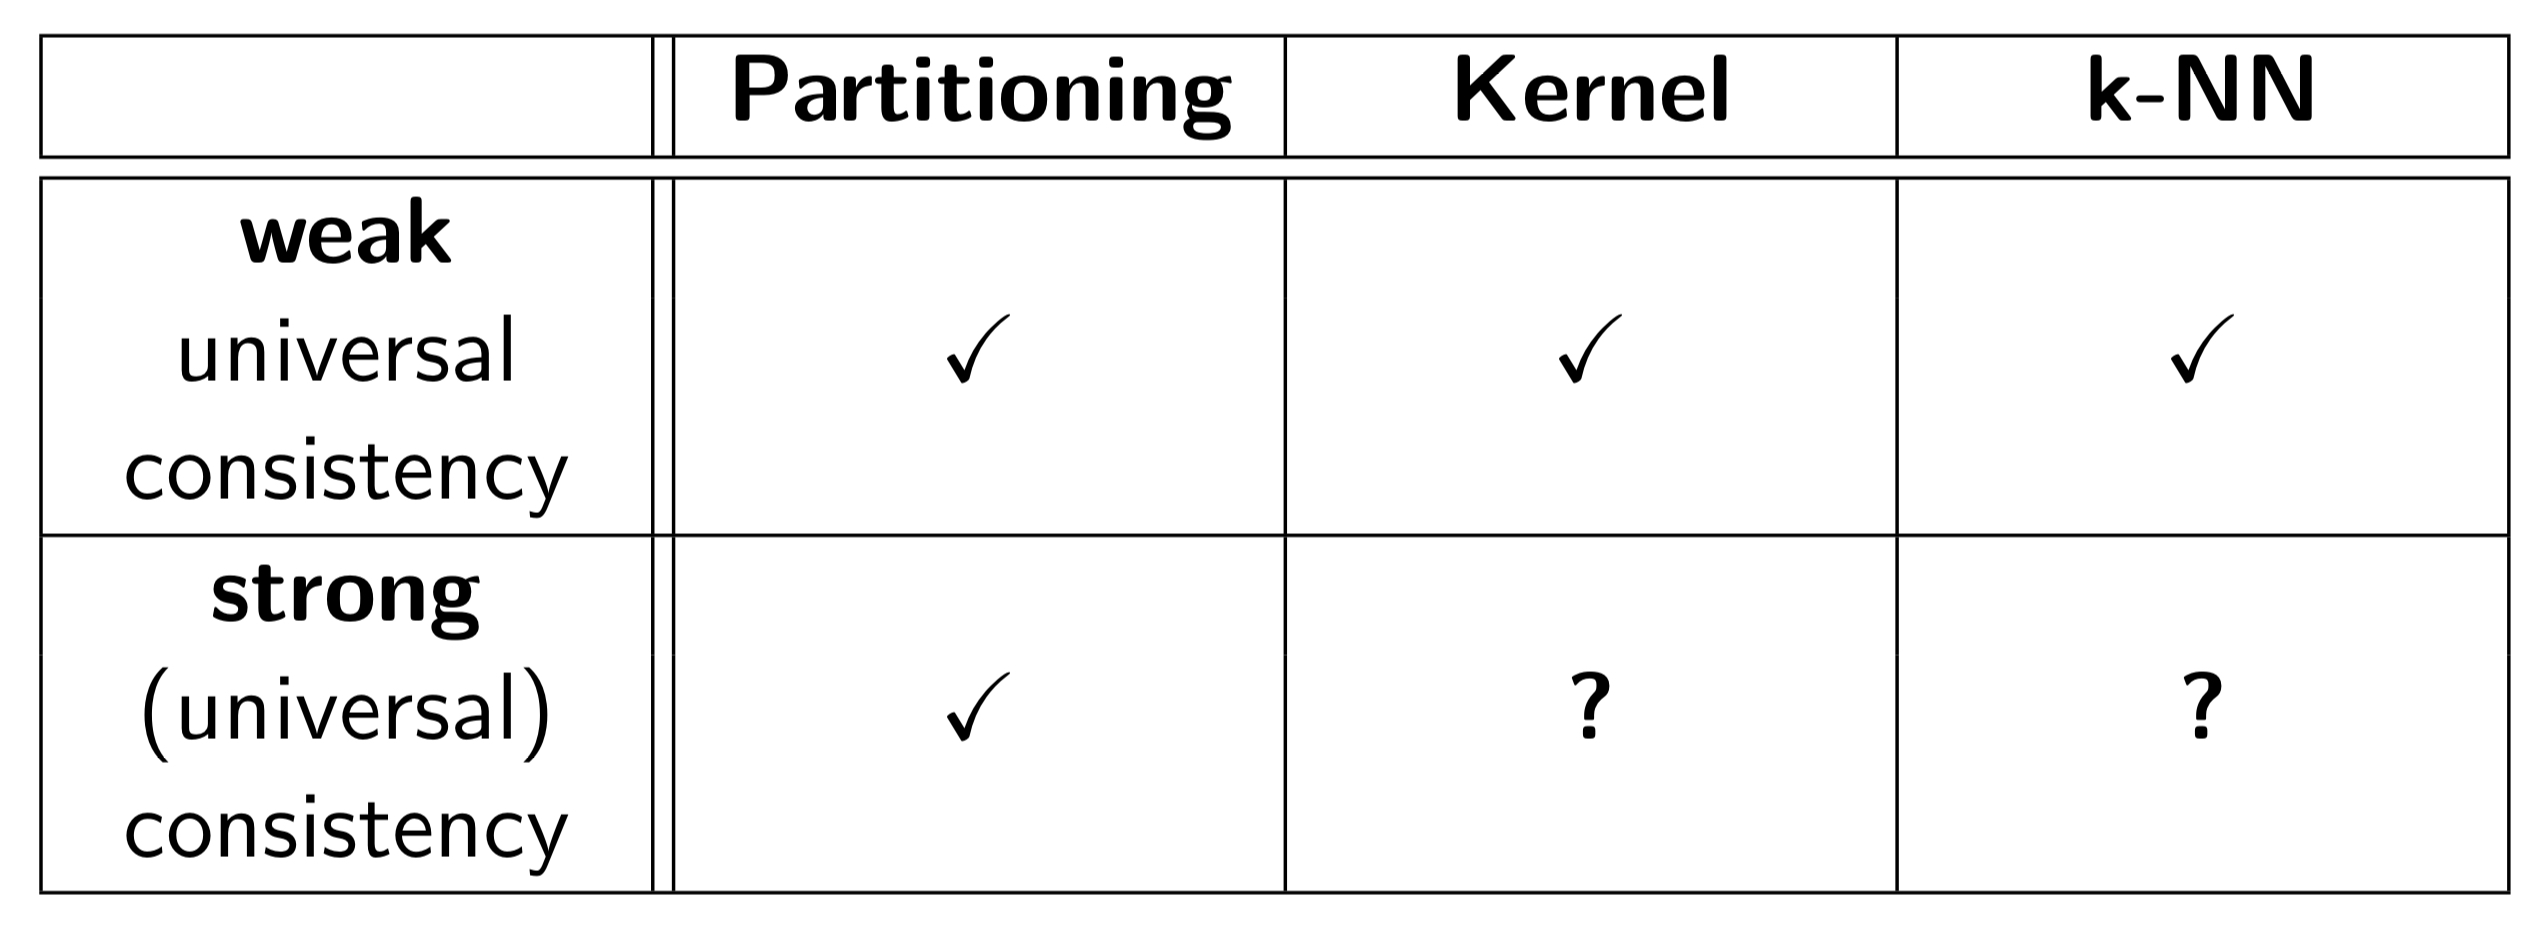
\includegraphics[scale=0.12]{wherearewe.jpeg}
    \centering
    \caption{Current position regarding to our content.}
\end{figure}


\begin{definition}[kernel estimate]
    Let $K: \: \R^d \to \R_{+}$ be a function called kernel function, and let $h>0$ be a bandwidth. The kernel estimate is defined by
    \[m_n(x) = \frac{\sum_{i=1}^nK(\frac{x-X_i}{h})Y_i}{\sum_{i=1}^nK(\frac{x-X_i}{h})}.\]
\end{definition}

\begin{definition}[$k$-NN estimate]
    For $x \in \R^d$ let
    \[(X_{(1)}(x),Y_{(1)}(x)),...,(X_{(n)}(x),Y_{(n)}(x))\]
    be a permutation of
    \[(X_1,Y_2),...,(X_n,Y_n)\]
    such that
    \[\norm{x-X_{(1)}(x)} \leq ... \leq \norm{x-X_{(n)}(x)}.\]
    The $k$-NN estimate is defined by
    \[m_n(x) = \frac{1}{k} \sum_{i=1}^kY_{(i)}(x).\]
\end{definition}

\begin{definition}[strong universal consistency]
    A sequence of regression function estimates $\{m_n\}_n$ is called strongly consistent for a certain distribution of $(X,Y)$, if
    \[\limn \int \abs{m_n(x) - m(x)}^2 \mu(\diff{x}) = 0 \quad\text{with probability one.}\]
    This sequence is called strongly universal consistent if it is strongly consistent for all distributions of $(X,Y)$ with $\ev{Y^2}<\infty$.
\end{definition}

%-------------------------------------------------------------------
\newpage
%-------------------------------------------------------------------

% Table of contents in "Kernel estimates"
% Definition 23.1 (regular kernels)
% Lemma 23.6 + proof
% Lemma 23.7 + proof
% Lemma 23.8 + proof
% Lemma 23.9 + proof
% Theorem 23.5 + proof
% Lemma 23.3 (without proof: not in our section)
% Lemma 23.5 (without proof: not in our section)
% Theorem 23.6 + proof

\section{Kernel Estimates} \label{kernelestimates}

In this section we are going to proof the strong consistency for the kernel estimate. Therefore, we consider a rather general class of kernels. 

\begin{definition}[regular kernel] \label{defregularkernel}
A kernel is called regular if it is non-negative, and there exists a ball $B_r(0)$ with radius $r>0$ and a constant $b>0$ such that \[ 1 \geq K(x) \geq b \ind{\{x \in B_r(0)\}} \] and \begin{equation} \label{defregularkerneleq}
    \int \sup\limits_{u \in x+B_r(0)} K(u) \dx < \infty.
    \end{equation}
\end{definition}

\begin{figure}[h] 
    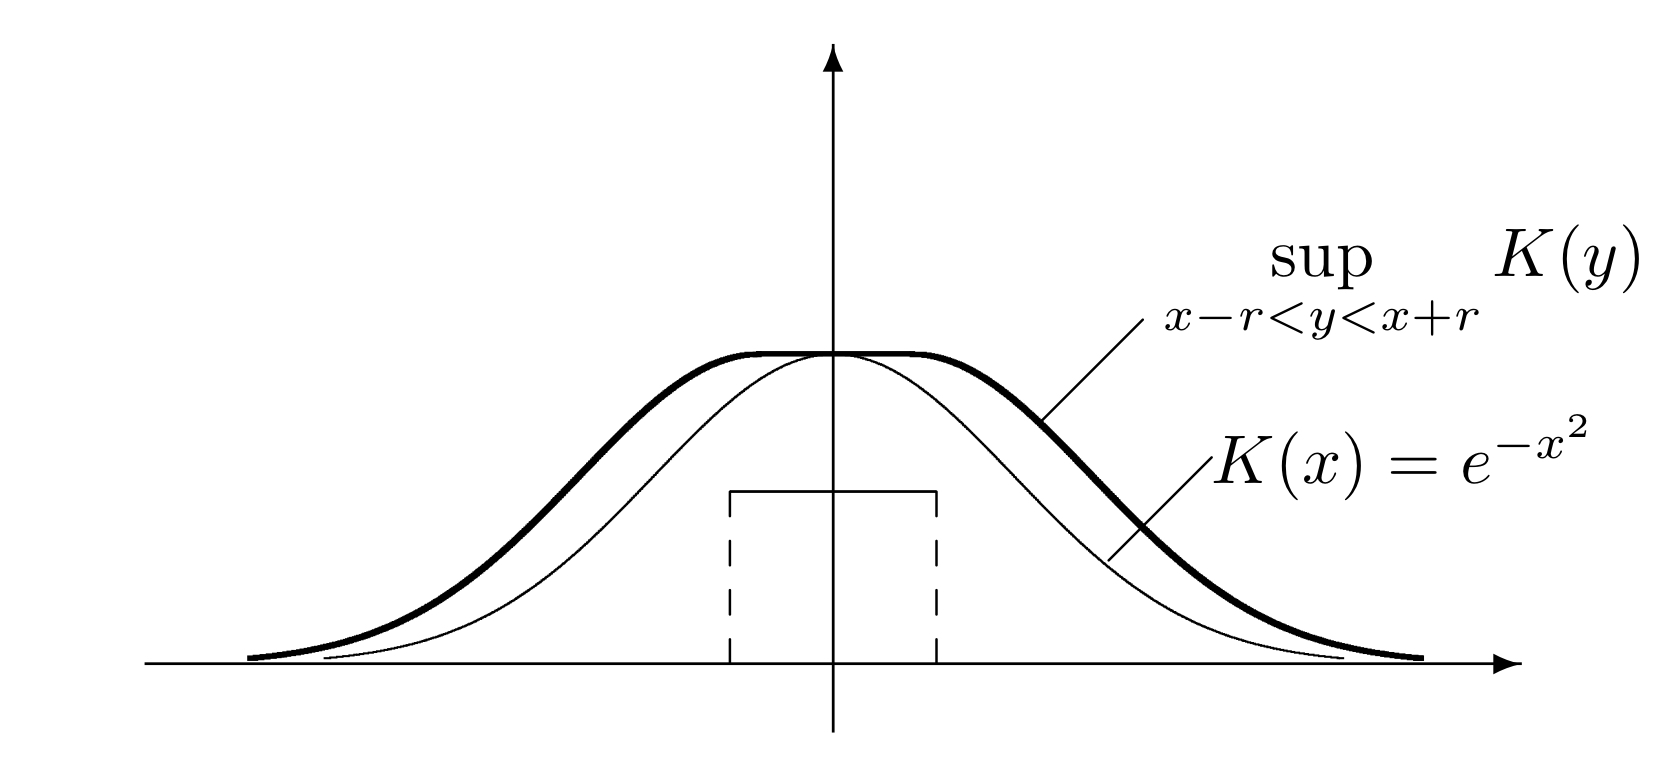
\includegraphics[scale=0.18]{regularKernelFigure.jpeg}
    \centering
    \caption{Regular kernel.} \label{figregularkernel}
\end{figure}

Put $K_h(x) := K(\frac{x}{h})$.

The following organizational chart (Figure \ref{chartkernelproof}) is intended to provide an overview of the structure of the proof of theorem \ref{kernelsc}, in order to better understand the organization and connections of the individual proof components.

\begin{figure}[h] 
    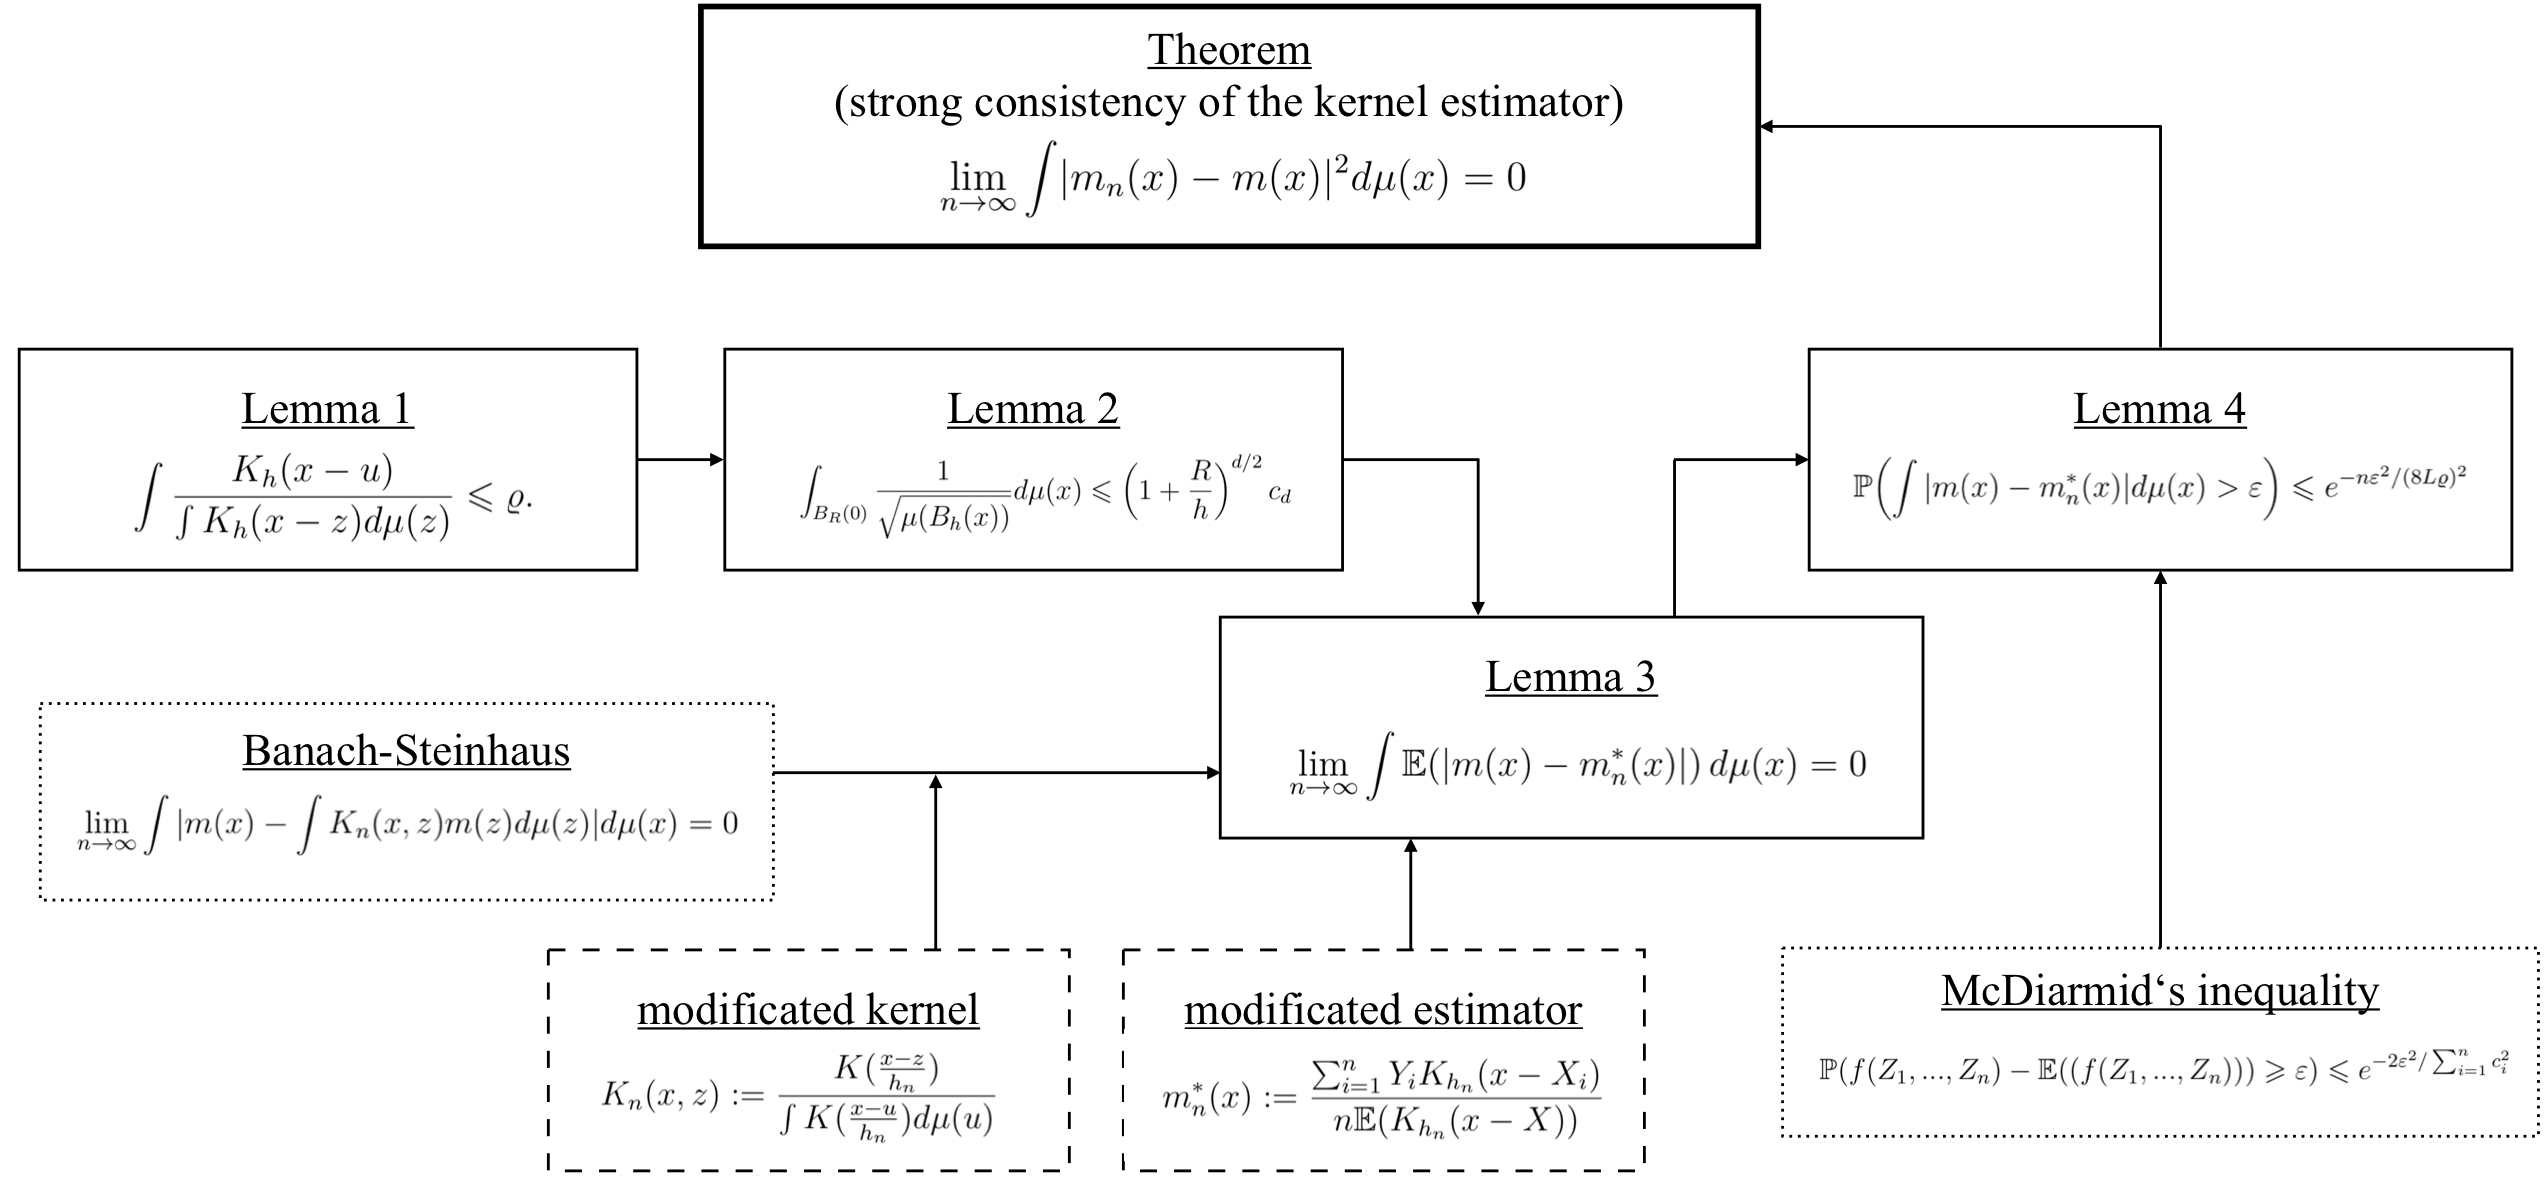
\includegraphics[scale=0.155]{organigramkernel.jpeg}
    \centering
    \caption{Organizational chart of the proof of theorem \ref{kernelsc}.} \label{chartkernelproof}
\end{figure}

%%% Lemma 23.6 (Covering Lemma)
\begin{lemma}[Covering Lemma] \label{coveringlemma}
If the kernel is regular then there exists a constant $\rho \equiv \rho(K)<\infty$ such that for any $u \in \mathbb{R}^d$, $h>0$ and every probability measure $\mu$ \[\int \frac{K_h(x-u)}{\int K_h(x-z) \mu(\diff{z})} \mu(\dx) \leq \rho.\]
Moreover, for any $\delta > 0$ \[\lim_{n\to\infty} \sup\limits_{u \in \mathbb{R}^d} \int \frac{K_h(x-u) \ind{\{ \| x-u \| > \delta \} }}{\int K_h(x-z) \mu(\diff{z})} \mu(\dx) = 0.\]
\end{lemma}

\begin{figure}[h] 
    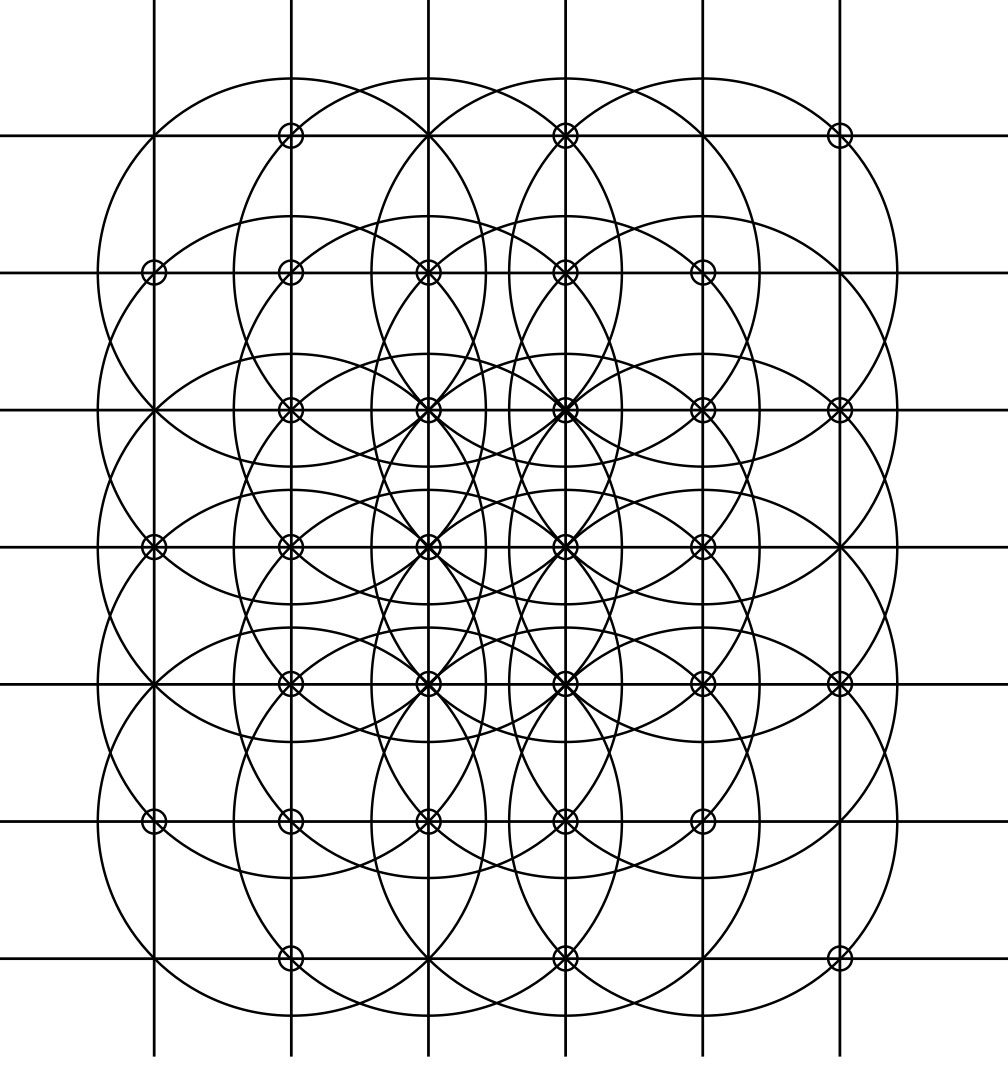
\includegraphics[scale=0.18]{coverofR2.jpeg}
    \centering
    \caption{An example of a bounded overlap of $\R^2$.} \label{figboundedoverlap}
\end{figure}

% proof of Lemma 23.6
\begin{proof}
    The kernel is regular which especially implies the existence of $r>0$ and $b>0$ such that \[ 1 \geq K(x) \geq b \ind{\{x \in B_r(0)\}}. \]
    Hence, there exists a bounded covering of $\R^d$ of balls with radius $\frac{r}{2}$ and centers $x_i$ $(i=1,2,...)$, i.e.\@
    $$\R^d = \bigcup_{i \in \N} B_{r/2}(x_i).$$
    This cover has an infinite number of member balls, but every $x$ gets covered at most $k_1$ times (see Figure \ref{figboundedoverlap}), where $k_1$ depends upon $d$ only, which implies
    \begin{equation} \label{coverofk1}
        \sum_{i=1}^\infty \ind{\{x \in B_{r/2}(x_i)\}} \leq k_1. 
    \end{equation}
    The integral condition (\ref{defregularkerneleq}) on $K$ implies that
    \begin{align} \label{leqk2}
        &\sum_{i=1}^\infty \sup\limits_{z\in B_{r/2}(x_i)} K(z) \\ 
        &= \sum_{i=1}^\infty \sup\limits_{z\in B_{r/2}(x_i)} K(z) \cdot \frac{\int_{\{x \in B_{r/2}(x_i)\}} \dx}{\int_{\{x \in B_{r/2}(0)\}} \dx} \quad\text{(by translation invariance)} \nonumber \\
        &= \sum_{i=1}^\infty \frac{1}{\int_{B_{r/2}(0)} \dx} \int_{\{x \in B_{r/2}(x_i)\}} \sup\limits_{z\in B_{r/2}(x_i)} K(z) \dx \nonumber\\
        &= \frac{1}{\int_{B_{r/2}(0)} \dx} \int \sum_{i=1}^\infty \ind{\{x \in B_{r/2}(x_i)\}} \sup\limits_{z\in B_{r/2}(x_i)} K(z) \dx \quad\text{(by Fubini's theorem)} \nonumber\\
        &\leq \frac{1}{\int_{B_{r/2}(0)}\dx} \int \sum_{i=1}^\infty \ind{\{x \in B_{r/2}(x_i)\}} \sup\limits_{z\in B_{r}(x)} K(z) \dx  \nonumber \\ &\quad\quad\quad\quad\quad\quad\quad\quad\quad\quad \text{(because $x\in B_{r/2}(x_i) \Rightarrow B_{r/2}(x_i) \subseteq B_r(x)$)} \nonumber\\
        &\leq \frac{k_1}{\int_{B_{r/2}(0)} \dx} \int \sup\limits_{z \in B_r(x)} K(z) \dx \quad \text{(because of (\ref{coverofk1}))} \nonumber\\
        &\leq k_2 \quad \text{(because of (\ref{defregularkerneleq}))} \nonumber
    \end{align}
    for another finite constant $k_2$. Furthermore,
    \begin{align*}
        K_h(x-u)
        &= K\Bigl(\frac{x-u}{h}\Bigr) \quad\text{(by definition)}\\
        &\leq \sum_{i=1}^\infty \sup\limits_{\frac{x-u}{h} \in B_{r/2}(x_i)} K\Bigl(\frac{x-u}{h}\Bigr) \\
        &= \sum_{i=1}^\infty \sup\limits_{x \in u+hB_{r/2}(x_i)} K_h(x-u)
    \end{align*}
    and, for $x \in u+hB_{r/2}(x_i)$,
    \begin{align} \label{btimesmu}
        \int K_h(x-z) \mu(\diff{z})
        &= \int K\Bigl(\frac{x-z}{h}\Bigr) \mu(\diff{z}) \\
        &\geq \int b \cdot \ind{\{ \frac{x-z}{h} \in B_r(0) \}} \mu(\diff{z}) \nonumber \\ &\quad\text{(by definition of regular kernels)} \nonumber \\
        &= b \cdot \int \ind{\{ z \in x+hB_r(0) \}} \mu(\diff{z}) \nonumber \\
        &= b \cdot \mu(x+hB_r(0)) \nonumber \\ 
        &\geq b \cdot \mu(u+hB_{r/2}(x_i)), \quad\text{(because $x \in u+hB_{r/2}(x_i)$)}\nonumber   
    \end{align}
    from which we conclude
    \begin{align*}
        &\int \frac{K_h(x-u)}{\int K_h(x-z) \mu(\diff{z})} \mu(\diff{x}) \\
        &\leq \sum_{i=1}^\infty \int_{\{ x \in u+hB_{r/2}(x_i) \}} \frac{K_h(x-u)}{\int K_h(x-z) \mu(\diff{z})} \mu(\diff{x}) \quad \text{(because of the covering)} \\
        &\leq \sum_{i=1}^\infty \int_{\{ x \in u+hB_{r/2}(x_i) \}} \frac{ \sup_{z\in hB_{r/2}(x_i)} K_h(z) }{\int K_h(x-z) \mu(\diff{z})} \mu(\diff{x}) \quad \text{(because of the choice of x)} \\
        &\leq \sum_{i=1}^\infty \int_{\{ x \in u+hB_{r/2}(x_i) \}} \frac{ \sup_{z\in hB_{r/2}(x_i)} K_h(z) }{b \cdot \mu(u+hB_{r/2}(x_i))} \mu(\diff{x}) \quad \text{(because of (\ref{btimesmu}))} \\
        &= \sum_{i=1}^\infty \frac{ \sup_{z\in hB_{r/2}(x_i)} K_h(z) }{b \cdot \mu(u+hB_{r/2}(x_i))} \cdot \mu(u+hB_{r/2}(x_i)) \\
        &= \frac{1}{b} \sum_{i=1}^\infty \sup\limits_{z\in hB_{r/2}(x_i)} K_h(z) \\
        &\leq \frac{k_2}{b} \quad\text{(by (\ref{leqk2}))},
    \end{align*}
    where $k_2$ depends on $K$ and $d$ only. Define $\rho := \frac{k_2}{b}$ and get the first statement. \\
    To obtain the second statement in the lemma, substitute $K_h(z)$ above by $K_h(z) \ind{\{\norm{z}>\delta\}}$ for $\delta > 0$, which implies
    \begin{align*}
        & \sup\limits_{u \in \mathbb{R}^d} \int \frac{K_h(x-u) \ind{\{ \| x-u \| > \delta \} }}{\int K_h(x-z) \mu(\diff{z})} d \mu (x) \\
        &\leq \sup\limits_{u \in \mathbb{R}^d} \frac{1}{b} \sum_{i=1}^\infty \sup_{z\in hB_{r/2}(x_i)} K_h(z) \ind{\{ \norm{z} > \delta \}} \quad \text{(by above)} \\
        &= \sup\limits_{u \in \mathbb{R}^d} \frac{1}{b} \sum_{i=1}^\infty \sup_{z\in B_{r/2}(x_i)} K(z) \ind{\{ \norm{z} > \delta/h \}} \\
        &\longrightarrow 0
    \end{align*}
    as $h \rightarrow 0$ by dominated convergence.
\end{proof}

% Lemma 23.7
\begin{lemma} \label{lemma23.7}
Let $1 \leq R < \infty, 0<h \leq R$ and let $B_R(0) \subseteq \mathbb{R}^d$ be a ball of radius $R$. Then, for every probability measure $\mu$, 
\[\int_{B_R(0)} \frac{1}{\sqrt{\mu(B_h(x))}} \mu(\diff{x}) \leq \left(1+\frac{R}{h}\right)^{d/2} c_d,\]
where $c_d$ depends upon the dimension d only.
\end{lemma}
% proof of Lemma 23.7
\begin{proof}
    Let $1 \leq R < \infty, 0<h \leq R$. Hence, there exists $M \in \N$ with
    \[
        M \leq \frac{c_d'}{h^d} \leq \frac{c_d'}{\left( \frac{h}{h+R} \right)^d} = c_d' \left( \frac{h+R}{h} \right)^d
    \] for a constant $c_d'$ which depends on the dimension $d$ only, such that
    \[B_h(0) \subseteq \bigcup_{j=1}^{M} B_{h/2}(z_j)\]
    with centers $z_1,...,z_{M}$. Therefore, by the Cauchy-Schwarz inequality
    \begin{align*}
        \int_{B_R(0)} \frac{1}{\sqrt{\mu(B_h(x))}} \mu(\diff{x})
        &\leq \left( \int_{B_R(0)} \frac{1}{\mu(B_h(x))} \mu(\diff{x}) \right)^\frac{1}{2} \\
        &\leq \left( \sum_{j=1}^{M} \int \frac{\ind{\{x \in B_{h/2}(z_j)\}}}{\mu(B_h(x))} \mu(\diff{x}) \right)^\frac{1}{2} \\
        &\leq \left( \sum_{j=1}^{M} \int \frac{\ind{\{x \in B_{h/2}(z_j)\}}}{\mu(B_{h/2}(z_j))} \mu(\diff{x}) \right)^\frac{1}{2} \\
        &\leq \left( \sum_{j=1}^{M} 1 \right)^\frac{1}{2} \\
        &= M^\frac{1}{2} \\
        &\leq \left( c_d' \left( \frac{h+R}{h} \right)^d \right)^\frac{1}{2} \\
        &= \left(1+\frac{R}{h}\right)^{d/2} \underset{:= \sqrt{c_d'}}{\underbrace{c_d}}.
    \end{align*}
\end{proof}

Define \[m_n^*(x) := \frac{\sum_{i=1}^{n} Y_i K_{h_n}(x-X_i)}{n \ev{K_{h_n}(x-X)}}. \]

% Lemma 23.8
\begin{lemma} \label{lemma23.8}
Let $m_n$ be the kernel estimate of the regression function m with a regular kernel K. Assume that there is an $L<\infty$ such that $P(|Y| \leq L) = 1.$ If \[h_n \to 0 \quad and \quad nh_n^d \to \infty,\] then we have
\[\lim_{n\to\infty} \int \ev{|m(x) - m_n^*(x)|} \mu(\diff{x}) = 0.\]
\end{lemma}
% proof of Lemma 23.8
\begin{proof}
    By the triangle inequality
    \begin{align*}
        &\int \ev{|m(x)-m_n^*(x)|}\mu(\diff{x}) \\
        &= \int \ev{|m(x)-\ev{m_n^*(x)}+\ev{m_n^*(x)}-m_n^*(x)|}\mu(\diff{x}) \\
        &\leq \int \ev{|m(x)-\ev{m_n^*(x)}|}\mu(\diff{x}) + \int \ev{|\ev{m_n^*(x)}-m_n^*(x)|}\mu(\diff{x}) \\
        &=: I_n + J_n.
    \end{align*}
    Concerning the term $I_n$ verify the conditions of the Theorem of Banach-Steinhaus (Appendix, Theorem \ref{banachsteinhaus}) for
    \[K_n(x,z) := \frac{K(\frac{x-z}{h_n})}{\int K(\frac{x-u}{h_n}) \mu(\diff{u})}.\]
    By this definition, we have
    \begin{align} \label{expofmn*}
        \ev{m_n^*(x)}
        &= \ev{\frac{\sum_{i=1}^{n} Y_i K_{h_n}(x-X_i)}{n E(K_{h_n}(x-X))}} \quad\text{(by definition)} \\
        &= \frac{1}{n \ev{K_{h_n}(x-X)}} n\ev{Y K_{h_n}(x-X)} \quad\text{($X,X_1,X_2,...$ iid.)} \nonumber \\ 
        &= \frac{\ev{YK_{h_n}(x-X)}}{\ev{K_{h_n}(x-X)}} \nonumber \\
        &= \frac{\ev{\ev{Y K_{h_n}(x-X)|X}}}{\ev{K_{h_n}(x-X)}} \quad\text{(by tower property)} \nonumber \\
        &= \frac{\ev{K_{h_n}(x-X)\ev{Y|X}}}{\ev{K_{h_n}(x-X)}} \nonumber \\
        &= \frac{\ev{K_{h_n}(x-X)m(X)}}{\ev{K_{h_n}(x-X)}} \quad\text{(by the definition of $m$)}\nonumber \\
        &= \int \frac{K(\frac{x-z}{h_n})}{\int K(\frac{x-u}{h_n} \mu(\diff{u}))} m(z) \mu(\diff{z}) \nonumber \\
        &= \int K_n(x,z) m(z) \mu(\diff{z}). \quad\text{(by definition of $K_n$)}\nonumber 
    \end{align}
    Part (i) follows from the covering lemma with $c = \rho$: Let $z \in \R^d$. We get
    \begin{align*}
        \int |K_n(x,z)| \mu(\diff{x}) 
        &= \int \frac{K(\frac{x-z}{h_n})}{\int K(\frac{x-u}{h_n}) \mu(\diff{u})} \mu(\diff{x}) \quad\text{(by definition of $K_n$)} \\
        &= \int \frac{K_{h_n}(x-z)}{\int K_{h_n}(x-u) \mu(\diff{u}))} \mu(\diff{x}) \quad\text{(by $K_h(x):=K(x/h)$)} \\
        &\leq \rho. \quad \text{(by Lemma \ref{coveringlemma})}
    \end{align*}
    Part (ii) follows from the covering lemma with $d = \rho$: Let $x \in \R^d.$ Hence,
    \begin{align*}
        \int |K_n(x,z)| \mu(\diff{z}) 
        &= \int \frac{K(\frac{x-z}{h_n})}{\int K(\frac{z-u}{h_n}) \mu(\diff{u})} \mu(\diff{z}) \quad\text{(by definition of $K_n$)} \\
        &= \int \frac{K_{h_n}(x-z)}{\int K_{h_n}(z-u) \mu(\diff{u}))} \mu(\diff{z}) \quad\text{(by $K_h(x):=K(x/h)$)} \\
        &\leq \rho. \quad \text{(by Lemma \ref{coveringlemma})}
    \end{align*}
    Let $a>0$. We get part (iii) by
    \begin{align*}
        & \int \int K_n(x,z) \ind{\{\norm{x-z}>a\}} \mu(\diff{z}) \mu(\diff{x}) \\
        &= \int \int \frac{K(\frac{x-z}{h_n})}{\int K(\frac{x-u}{h_n} \mu(\diff{u}))} \ind{\{\norm{x-z}>a\}} \mu(\diff{z}) \mu(\diff{x}) \quad\text{(by definition of $K_n$)} \\
        &= \int \frac{\int K(\frac{x-z}{h_n}) \ind{\{\norm{x-z}>a\}} \mu(\diff{z})}{\int K(\frac{x-u}{h_n}) \mu(\diff{u})} \mu(\diff{x}) \\
        &= \int \frac{\int K_{h_n}(x-z) \ind{\{\norm{x-z}>a\}} \mu(\diff{z})}{\int K_{h_n}(x-u) \mu(\diff{u})} \mu(\diff{x})\\
        &\longrightarrow 0 
    \end{align*}
    by the second statement of the covering lemma (\ref{coveringlemma}) by using $a$ instead of $\delta$.\\
    Part (iv) is obvious since
    \begin{align*}
        ess\sup\limits_{x \in \R^d} \int K_n(x,z) \mu(\diff{z})
        = ess\sup\limits_{x \in \R^d} \frac{\int K(\frac{x-z}{h_n}) \mu(\diff{z})}{\int K(\frac{x-u}{h_n}) \mu(\diff{u})}
        = ess\sup\limits_{x \in \R^d} 1
        = 1.
    \end{align*}
    By applying the theorem of Banach-Steinhaus (Appendix, \ref{banachsteinhaus}) we get
    \begin{align*}
        &\int \ev{|m(x)-\ev{m_n^*(x)}|}\mu(\diff{x}) \\
        &= \int \ev{|m(x)-\int K_n(x,z)m(z)\mu(\diff{z})|}\mu(\diff{x}) \quad\text{(by (\ref{expofmn*}))} \\
        & \longrightarrow 0.
    \end{align*}

    For the second term $J_n$ we have with $h = h_n$ for convenience,
    \begin{align*}
        &\ev{|m_n^*(x)-E(m_n^*(x))|} \\
        &= \sqrt{\ev{|m_n^*(x)-\ev{m_n^*(x)}|^2}} \quad\text{(by Cauchy-Schwarz)} \\
        &= \sqrt{\ev{\abs[\bigg]{\frac{\sum_{i=1}^n Y_i K_h(x-X_i)}{n\ev{K_n(x-X_i)}} - \ev{\frac{\sum_{i=1}^n Y_i K_h(x-X_i)}{n\ev{K_n(x-X_i)}}}}^2}} \quad\text{(by definition)}\\
        &=\sqrt{\ev{\abs[\bigg]{\frac{nYK_h(x-X)-n\ev{YK_h(x-X)}}{n\ev{K_h(x-X)}}}^2}} \quad\text{($X,X_1,X_2,...$ iid)} \\
        &=\sqrt{\frac{n \ev{|YK_h(x-X)-\ev{YK_h(x-X)|}^2}}{n^2 \ev{K_h(x-X)})^2}} \\ 
        &=\sqrt{\frac{\ev{|YK_h(x-X)-\ev{YK_h(x-X)|^2}}}{n \ev{K_h(x-X)}^2}} \\ 
        &\leq \sqrt{\frac{\ev{|YK_h(x-X)|^2}}{n \ev{K_h(x-X)}^2}} \quad\text{(by definition of the variance: $\ev{YK_h(x-X)} \geq 0$)} \\
        &\leq L \sqrt{\frac{\ev{|K_h(x-X)|^2}}{n \ev{K_h(x-X)}^2}} \quad\text{(since $|Y|\leq L$)}\\
        &\leq L \sqrt{\frac{\ev{|K(\frac{x-X}{h})|^2}}{n \ev{K(\frac{x-X}{h})}^2}} \quad\text{(by $K_h(x):= K(x/h)$)}\\
        &\leq L \sqrt{K_{max}} \sqrt{\frac{\ev{K(\frac{x-X}{h})}}{n \ev{K(\frac{x-X}{h})}^2}} \\
        &\leq L \sqrt{\frac{K_{max}}{b}} \sqrt{\frac{1}{n\mu (B_h(x))}}, \quad\text{(by (\ref{btimesmu}))}
    \end{align*}
    where $K_{max}$ is a upper bound of $K$, i.e.\@ $K(x) \leq K_{max}$ $\forall x \in \R$ which is possible reasoned by the definition of regular kernels. \\
    Let $R>0$. Hence, we can split the integral such that
    \begin{align*}
        &\int_{\R^d} \ev{|m_n^*(x)-\ev{m_n^*(x)}|} \mu(\diff{x}) \\
        &= \int_{B_R(0)} \ev{|m_n^*(x)-\ev{m_n^*(x)}|} \mu(\diff{x}) + \int_{B_R(0)^c} \ev{|m_n^*(x)-\ev{m_n^*(x)}|} \mu(\diff{x}).
    \end{align*}
    For the integral outside the ball we have 
    \begin{align*}
        &\int_{B_R(0)^c} \ev{|m_n^*(x)-\ev{m_n^*(x)}|} \mu(\diff{x}) \\
        &\leq 2 \int_{B_R(0)^c} \ev{|m_n^*(x)|} \mu(\diff{x}) \quad\text{(by triangle inequality)}\\ 
        &\leq 2L \mu(B_R(0)^c) \quad\text{(by assumption $\abs{Y}\leq L$ and by definition of $m_n^*$)}\\
        &\longrightarrow 0
    \end{align*}
    since $R \rightarrow \infty$.\\
    To bound the integral over $B_R(0)$ we employ Lemma \ref{lemma23.7}:
    \begin{align*}
        &\int_{B_R(0)} \ev{|m_n^*(x)-\ev{m_n^*(x)}|} \mu(\diff{x}) \\
        &\leq \int_{B_R(0)} L \sqrt{\frac{K_{max}}{b}} \sqrt{\frac{1}{n\mu (B_h(x))}} \mu(\diff{x}) \quad\text{(by the inequality obtained above)} \\
        &= L \sqrt{\frac{K_{max}}{b}} \frac{1}{\sqrt{n}} \int_{B_R(0)} \sqrt{\frac{1}{\mu (B_h(x))}} \mu(\diff{x}) \\
        &\leq L \sqrt{\frac{K_{max}}{b}} \frac{1}{\sqrt{n}} \Bigl(1+\frac{R}{h}\Bigr)^{d/2} c_d \quad\text{(by Lemma \ref{lemma23.7})} \\
        &= L \sqrt{\frac{K_{max}}{b}} \Bigl(1+\frac{R}{hn^{1/d}}\Bigr)^{d/2} c_d \\
        &\longrightarrow 0 \quad\text{(by assumption $nh_n^d \rightarrow \infty$ and continuity)}.
    \end{align*}
    Therefore,
    \begin{align*}
        &\int \ev{|m(x)-m_n^*(x)|}\mu(\diff{x}) \\
        &\leq \int \ev{|m(x)-\ev{m_n^*(x)}|}\mu(\diff{x}) + \int \ev{\ev{m_n^*(x)}-m_n^*(x)|}\mu(\diff{x}) \\
        &\longrightarrow 0.
    \end{align*}
\end{proof}

% Lemma 23.9
\begin{lemma} \label{lemma23.9}
For n large enough \[\pro{\int |m(x) - m_n^*(x)| \mu(\diff{x}) > \epsilon} \leq e^{-n\epsilon^2/(8L\rho)^2}. \]
\end{lemma}
% proof of Lemma 23.9
\begin{proof}
    We use the decomposition
    \begin{align*}
        &\int |m(x)-m_n^*(x)| \mu(\diff{x}) \\
        &= \int \abs{m(x)-m_n^*(x)} - \ev{|m(x)-m_n^*(x)|} +  \ev{|m(x)-m_n^*(x)|} \mu(\diff{x}) \\
        &= \int \ev{|m(x)-m_n^*(x)|} \mu(\diff{x}) + \int |m(x)-m_n^*(x)| - \ev{|m(x)-m_n^*(x)|} \mu(\diff{x}).
    \end{align*}
    The first term on the right-hand side tends to $0$ by Lemma \ref{lemma23.8}. It remains to show that the second term on the right-hand side is small with large probability. To do this, we use McDiarmid's inequality (Appendix, \ref{mcdiarmidineq}) for
    \[\int |m(x)-m_n^*(x)| \mu(\diff{x}) - \ev{\int |m(x)-m_n^*(x)| \mu(\diff{x})}.\]
    Fix the training data at $((x_1,y_1),...,(x_n,y_n))$ and replace the $i$th pair $(x_i,y_i)$ by $(\hat{x_i},\hat{y_i})$, changing the value of $m_n^*(x)$ to $m_{ni}^*(x)$. 
    In detail, we consider the transformation \(T_i\) for \(i = 1,...,n\) defined as
    \[((x_1, y_1),...,(x_n, y_n)) \mapsto ((x_1, y_1),...,(x_{i-1}, y_{i-1}),(\hat{x_i}, \hat{y_i}),(x_{i+1}, y_{i+1}),...,(x_n, y_n))\]
    where $(\hat{x_i}, \hat{y_i}) \in \R^d \times \R$ . Hence,
\[m_{ni}^*(x, D_n(\omega)) = m_n^*(x, T_i(D_n(\omega))).\] 
    Clearly, by the covering lemma (Lemma \ref{coveringlemma}), we get for fixed training data, i.e.\@ \(\omega \in \Omega\) fixed,
    \begin{align*}
        &\int |m(x) - m_n^*(x)| \mu(\diff{x}) - \int |m(x) - m_{ni}^*(x)| \mu(\diff{x}) \\
        &= \int |m(x) - m_n^*(x)| - |m(x) - m_{ni}^*(x)| \mu(\diff{x}) \\
        &\leq \int |m(x) - m_n^*(x) - m(x) - m_{ni}^*(x)| \mu(\diff{x}) \quad\text{(by reverse triangle inequality)}\\
        &= \int |m_n^*(x) - m_{ni}^*(x)| \mu(\diff{x}) \\
        &= \int \abs[\bigg]{\frac{\sum_{j=1}^{n} y_j K_{h_n}(x-x_j)}{n \ev{K_{h_n}(x-X)}} - \frac{\hat{y_i} K_{h_n}(x - \hat{x_i}) + \sum_{j\neq i}^{n} y_j K_{h_n}(x-x_j)}{n \ev{K_{h_n}(x-X)}}} \mu(\diff{x}) \quad\text{(by definition)} \\
        &= \int \abs[\bigg]{\frac{y_i K_{h_n}(x-x_i) - \hat{y_i} K_{h_n}(x-\hat{x_i})}{n \ev{K_{h_n}(x-X)}}} \mu(\diff{x}) \quad\text{(by definition)} \\
        &\leq \sup\limits_{y\in \R^d} \int \frac{2LK_{h_n}(x-y)}{n\ev{K_{h_n}(x-X)}} \mu(\diff{x}) \\
        &= \frac{2L}{n} \sup\limits_{y\in \R^d} \int \frac{K_{h_n}(x-y)}{\int K_{h_n}(x-z) \mu(\diff{z})} \mu(\diff{x})\\
        &\leq \frac{2L\rho}{n}. \quad\text{(by Lemma \ref{coveringlemma})}
    \end{align*}
    So by Theorem \ref{mcdiarmidineq}, for $n$ large enough we get 
    \[
        I_n := \ev{\int |m(x)-m_n^*(x)| \mu(\diff{x})} < \frac{\epsilon}{2} \quad\text{(by Lemma \ref{lemma23.8})}.
    \]
     We notice that for random Variables \(A, B, C\), we have that
    \begin{align} \label{probeq1}
        \pro{B > C} \leq \pro{A > C} \quad \text{if \(A \geq B\)},
    \end{align}
    and thus
    \begin{align*}
        &\pro{\int |m(x) - m_n^*(x)| \mu(\diff{x}) > \epsilon} \\ 
        &= \pro{\int |m(x) - m_n^*(x)| \mu(\diff{x}) - I_n > \epsilon - I_n} \\
        &\leq \pro{\int |m(x) - m_n^*(x)| \mu(\diff{x}) - \ev{\int |m(x)-m_n^*(x)| \mu(\diff{x})}  > \frac{\epsilon}{2}} \\ 
        &\leq e^{-2\frac{(\epsilon/2)^2}{4L^2\rho^2}} \\
        &= e^{-n\epsilon^2/(8L^2\rho^2)}.
    \end{align*}
    The proof is now complete.
\end{proof}

% Theorem 23.5 (kernel est. sc)
\begin{theorem} \label{kernelsc}
Let $m_n$ be the kernel estimate of the regression function m with a regular kernel K. Assume that there is an $L<\infty$ such that $P(|Y| \leq L) = 1.$ If \[h_n \to 0 \quad and \quad nh_n^d \to \infty,\] then the kernel estimate is strongly consistent.
\end{theorem}
% proof of Theorem 23.5 (Kernel est. sc)
\begin{proof}
(proof of Theorem \ref{kernelsc}) It suffices to show that \[\lim_{n\to\infty} \int |m_n(x)-m(x)| \mu(\diff{x}) = 0,\quad \mathbb{P}\text{-a.s.}\] due to
\[
    \abs{m_n(x) - m(x)} \leq \abs{m_n(x)} + \abs{m(x)} \leq 2L
\]
and thus
\[
    \abs{m_n(x) - m(x)}^2 \leq 2L \abs{m_n(x) - m(x)}.
\]
With the triangle inequality we get the decomposition \[\int |m_n(x)-m(x)| \mu(\diff{x}) \leq \int |m_n(x)-m_n^*(x)| \mu(\diff{x}) + \int |m_n^*(x)-m(x)| \mu(\diff{x})\]
and, according to Lemma \ref{lemma23.9}, \[\int |m_n^*(x)-m(x)| \mu(\diff{x}) \to 0 \] with probability 1.
On the other hand, 
\begin{align*}
&\quad |m_n^*(x)-m_n(x)| \\
&= \abs[\bigg]{\frac{\sum_{i=1}^{n}Y_i K_{h_n}(x-X_i)}{n\ev{K_{h_n}(x-X)}} - 
\frac{\sum_{i=1}^{n}Y_i K_{h_n}(x-X_i)}{\sum_{i=1}^{n}K_{h_n}(x-X_i)}} \\
&= \abs[\Big]{\sum_{i=1}^{n}Y_i K_{h_n}(x-X_i)}
\abs[\bigg]{\frac{1}{n\ev{K_{h_n}(x-X)}} - \frac{1}{\sum_{i=1}^{n}K_{h_n}(x-X_i)}} \\
&\leq L \abs[\Big]{\sum_{i=1}^{n}K_{h_n}(x-X_i)}
\abs[\bigg]{\frac{1}{n\ev{K_{h_n}(x-X)}} - \frac{1}{\sum_{i=1}^{n}K_{h_n}(x-X_i)}} \\
&= L \abs[\bigg]{\frac{\sum_{i=1}^{n}Y_i K_{h_n}(x-X_i)}{n\ev{K_{h_n}(x-X)}} - 1} \\
&= L \abs{M_n^*(x)-1},
\end{align*}
where $M_n^*$ is a special form of $m_n^*(x)$ for $(X,1)$. \\\
In this case, $M(x) = \ev{Y|X=x} = \ev{1|X=x} = 1$ $ \forall x \in \mathbb{R}^d$ with $Y \equiv 1$.
Therefore, 
\[
\int|m_n^*(x)-m_n(x)| \mu(\diff{x}) \leq L \int |M_n^*(x)-1| \mu(\diff{x}) \to 0 \quad \mathbb{P}\text{-a.s.}
\]
which completes the proof.
\end{proof}

% ------
The subsequent lemmas help us to prove the following theorem which considers the strong universal consistency of the kernel estimate. These both lemmas will not be proved here. To review their proofs, please refer to section 23.1 of \textsc{Györfi}'s book.

% Lemma 23.3 (not in our section)
\begin{lemma} \label{lemma23.3}% page 466
Let $m_n$ be a local averaging regression function estimate with subprobability weights $\{\alpha_{n,i}(x)\}$ that is strongly consistent for all distributions of $(X,Y)$ such that $Y$ is bounded with probability one. Assume that there is a constant $c$ such that for all $Y$ with $\ev{Y^2}<\infty$,
\[\limsup_{n \to \infty} \sum_{i=1}^{n}Y_i^2 \int \alpha_{n,i}(x) \mu(\diff{x}) \leq c\ev{Y^2} \quad with \: probability \: one.\]
Then $m_n$ is strongly universally consistent.
\end{lemma}

% Lemma 23.5 (not in our section)
\begin{lemma} \label{lemma23.5} % page 473
Let $K_n$: $\mathbb{R}^d \times \mathbb{R}^d \to \{0,1\}$ be a measurable function. Assume that a constant $\rho>0$ exists with
\[\int \frac{K_n(x,z)}{\int K_n(x,s) \mu(\diff{s})} \mu(\diff{x}) \leq \rho\]
for all $n$, all $z$, and all distributions $\mu$. If $K_{n-1} \neq K_n$ at most for the indices $n=n_1,n_2,...,$ where $n_{k+1} \geq Dn_k$ for some fixed $D>1$, then
\[\limsup_{n\to\infty} \int \sum_{i=1}^{n} \frac{Y_i K_n(x,X_i)}{1+\sum_{j\in\{1,...,n\}\setminus\{i\}} K_n(x,X_j)} \mu(\diff{x}) \leq 2\rho \ev{Y} \quad\mathbb{P}\text{-a.s.},\]
for each integrable $Y\geq0.$
\end{lemma}

The following theorem concerns the strong universal consistency of the kernel estimate with naive kernel and a special sequence of bandwidths.
% Theorem 23.6 (kernel est. suc)
\begin{theorem} \label{kernelsuc}
Let $K(x) = \ind{\{\|x\|\leq1\}}$ and let $h_n$ satisfy 
\[h_{n-1} \neq h_n \quad \textit{at most for the indices} \ n=n_1,n_2,...,\]
where $n_{k+1} \geq Dn_k$ for fixed $D>1$. Additionally let 
\[ h_n \to 0 \quad and \quad nh_n^d \to \infty,\]
e.g., $h_n = ce^{-\gamma \lfloor q \log n \rfloor/q}$ with $c>0$, $0<\gamma d<1$ and $q>0$. Then $m_n$ is strongly universal consistent.
\end{theorem}

% proof of Theorem 23.6
\begin{proof} 
The assertion holds when there exists a $L>0$ with $|Y| \leq L$ (cf. Theorem \ref{kernelsc}).
According to Lemma \ref{lemma23.3}, it suffices to show, that for some constant $c>0$,
\begin{align*}
    c\ev{Y^2} 
    &\geq \limsup_{n\to\infty} \sum_{i=1}^{n} Y_i^2 \int \alpha_{ni}(x) \mu(\diff{x}) \\
    &= \limsup_{n\to\infty} \sum_{i=1}^{n} Y_i^2 \int \frac{K_{h_n}(x-X_i)}{\sum_{i=1}^n K_{h_n}(x-X_i)} \mu(\diff{x}) \quad\text{(by definition)}\\
    &= \limsup_{n\to\infty} \int \sum_{i=1}^{n} Y_i^2 \frac{K_{h_n}(x-X_i)}{\sum_{i=1}^n K_{h_n}(x-X_i)} \mu(\diff{x}), \quad\text{(by linearity of integrals)}\\
\end{align*}
$\mathbb{P}$-a.s., which is equivalent to
\begin{align*}
    &\limsup_{n\to\infty} \int \frac{\sum_{i=1}^{n}\abs{Y_i} K_{h_n}(x-X_i)}{\sum_{i=1}^{n}K_{h_n}(x-X_i)} \mu(\diff{x}) \\
    &= \limsup_{n\to\infty} \int \sum_{i=1}^{n} \frac{\abs{Y_i} K_n(x,X_i)}{\sum_{i=1}^{n}K_n(x,X_i)} \mu(\diff{x}) \\
    &= \limsup_{n\to\infty} \int \sum_{i=1}^{n} \frac{\abs{Y_i} K_n(x,X_i)}{1+\sum_{j\in\{1,...,n\}\setminus\{i\}} K_n(x,X_j)} \mu(\diff{x}) \\
    &\leq c\ev{\abs{Y}} \quad\text{$\mathbb{P}$-a.s.}
\end{align*}
with \(K_n(x, z) := K_{h_n}(x - z)\), 
for every distribution of $(X,Y)$ with $\ev{|Y|}<\infty$. This can be justified by Lemma \ref{lemma23.5}: Let $z \in \R^d$ and $n \in \N$. Hence,
\begin{align*}
    &\int \frac{K_n(x,z)}{\int K_n(x,s) \mu(\diff{s})} \mu(\diff{x}) \\
    %&= \int \frac{\frac{K(\frac{x-z}{h_n})}{\int K(\frac{x-u}{h_n}) \mu(\diff{u})}}{\int \frac{K(\frac{x-s}{h_n})}{\int K(\frac{x-u}{h_n}) \mu(\diff{u})} \mu(\diff{s})} \mu(\diff{x}) \quad\text{(by definition of $K_n$)} \\
    %&= \int \frac{K(\frac{x-z}{h_n})}{\int K(\frac{x-u}{h_n}) \mu(\diff{u})} \mu(\diff{x}) \\
    &= \int \frac{K_{h_n}(x-z)}{\int K_{h_n}(x-u) \mu(\diff{u}))} \mu(\diff{x}) \quad\text{(by definition)} \\
    &\leq \rho. \quad \text{(by Lemma \ref{coveringlemma})}
\end{align*}
With help of the assumption for the sequence of bandwidths of Theorem \ref{kernelsuc} we can apply Lemma \ref{lemma23.5} and get
\begin{align*}
    \limsup_{n\to\infty} \int \sum_{i=1}^{n} \frac{Y_i K_n(x,X_i)}{1+\sum_{j\in\{1,...,n\}\setminus\{i\}} K_n(x,X_j)} \mu(\diff{x}) 
    &\leq 2\rho \ev{Y} \quad\mathbb{P}\text{-a.s.}.
\end{align*}
for each integrable $Y\geq0$, which completes the proof.
\end{proof}

%-------------------------------------------------------------------
\newpage
%-------------------------------------------------------------------

\section{k-NN Estimates} \label{knnestimates}

Similar to Chapter \ref{kernelestimates}, we first of all proof the strong consistency of the $k$-NN estimates under certain assumptions and later on the strong universal consistency.


\begin{theorem}[strong consistency of the \(k\)-NN estimate] \label{knnsc}
Let \(\abs{Y} \leq L\) \(\mathbb{P}\)-a.s. for some \(L < \infty\) and that for each \(x \in \R^d\) the random variable \(\norm{X - x}\) is absolutely continuous, i.e.\@ its cumulative distribution function (CDF) is absolutely continuous. If \(k_n \to \infty\) and \(k_n / n \to 0\), then the \(k_n\)-NN regression function estimate is strongly consistent.
\end{theorem}

Analogous to the kernel estimate above, the following organizational chart (Figure \ref{chartknnproof}) is intended to illustrate the basic structure of the proof of Theorem \ref{knnsc}.

\begin{figure}[h] \label{chartknnproof}
    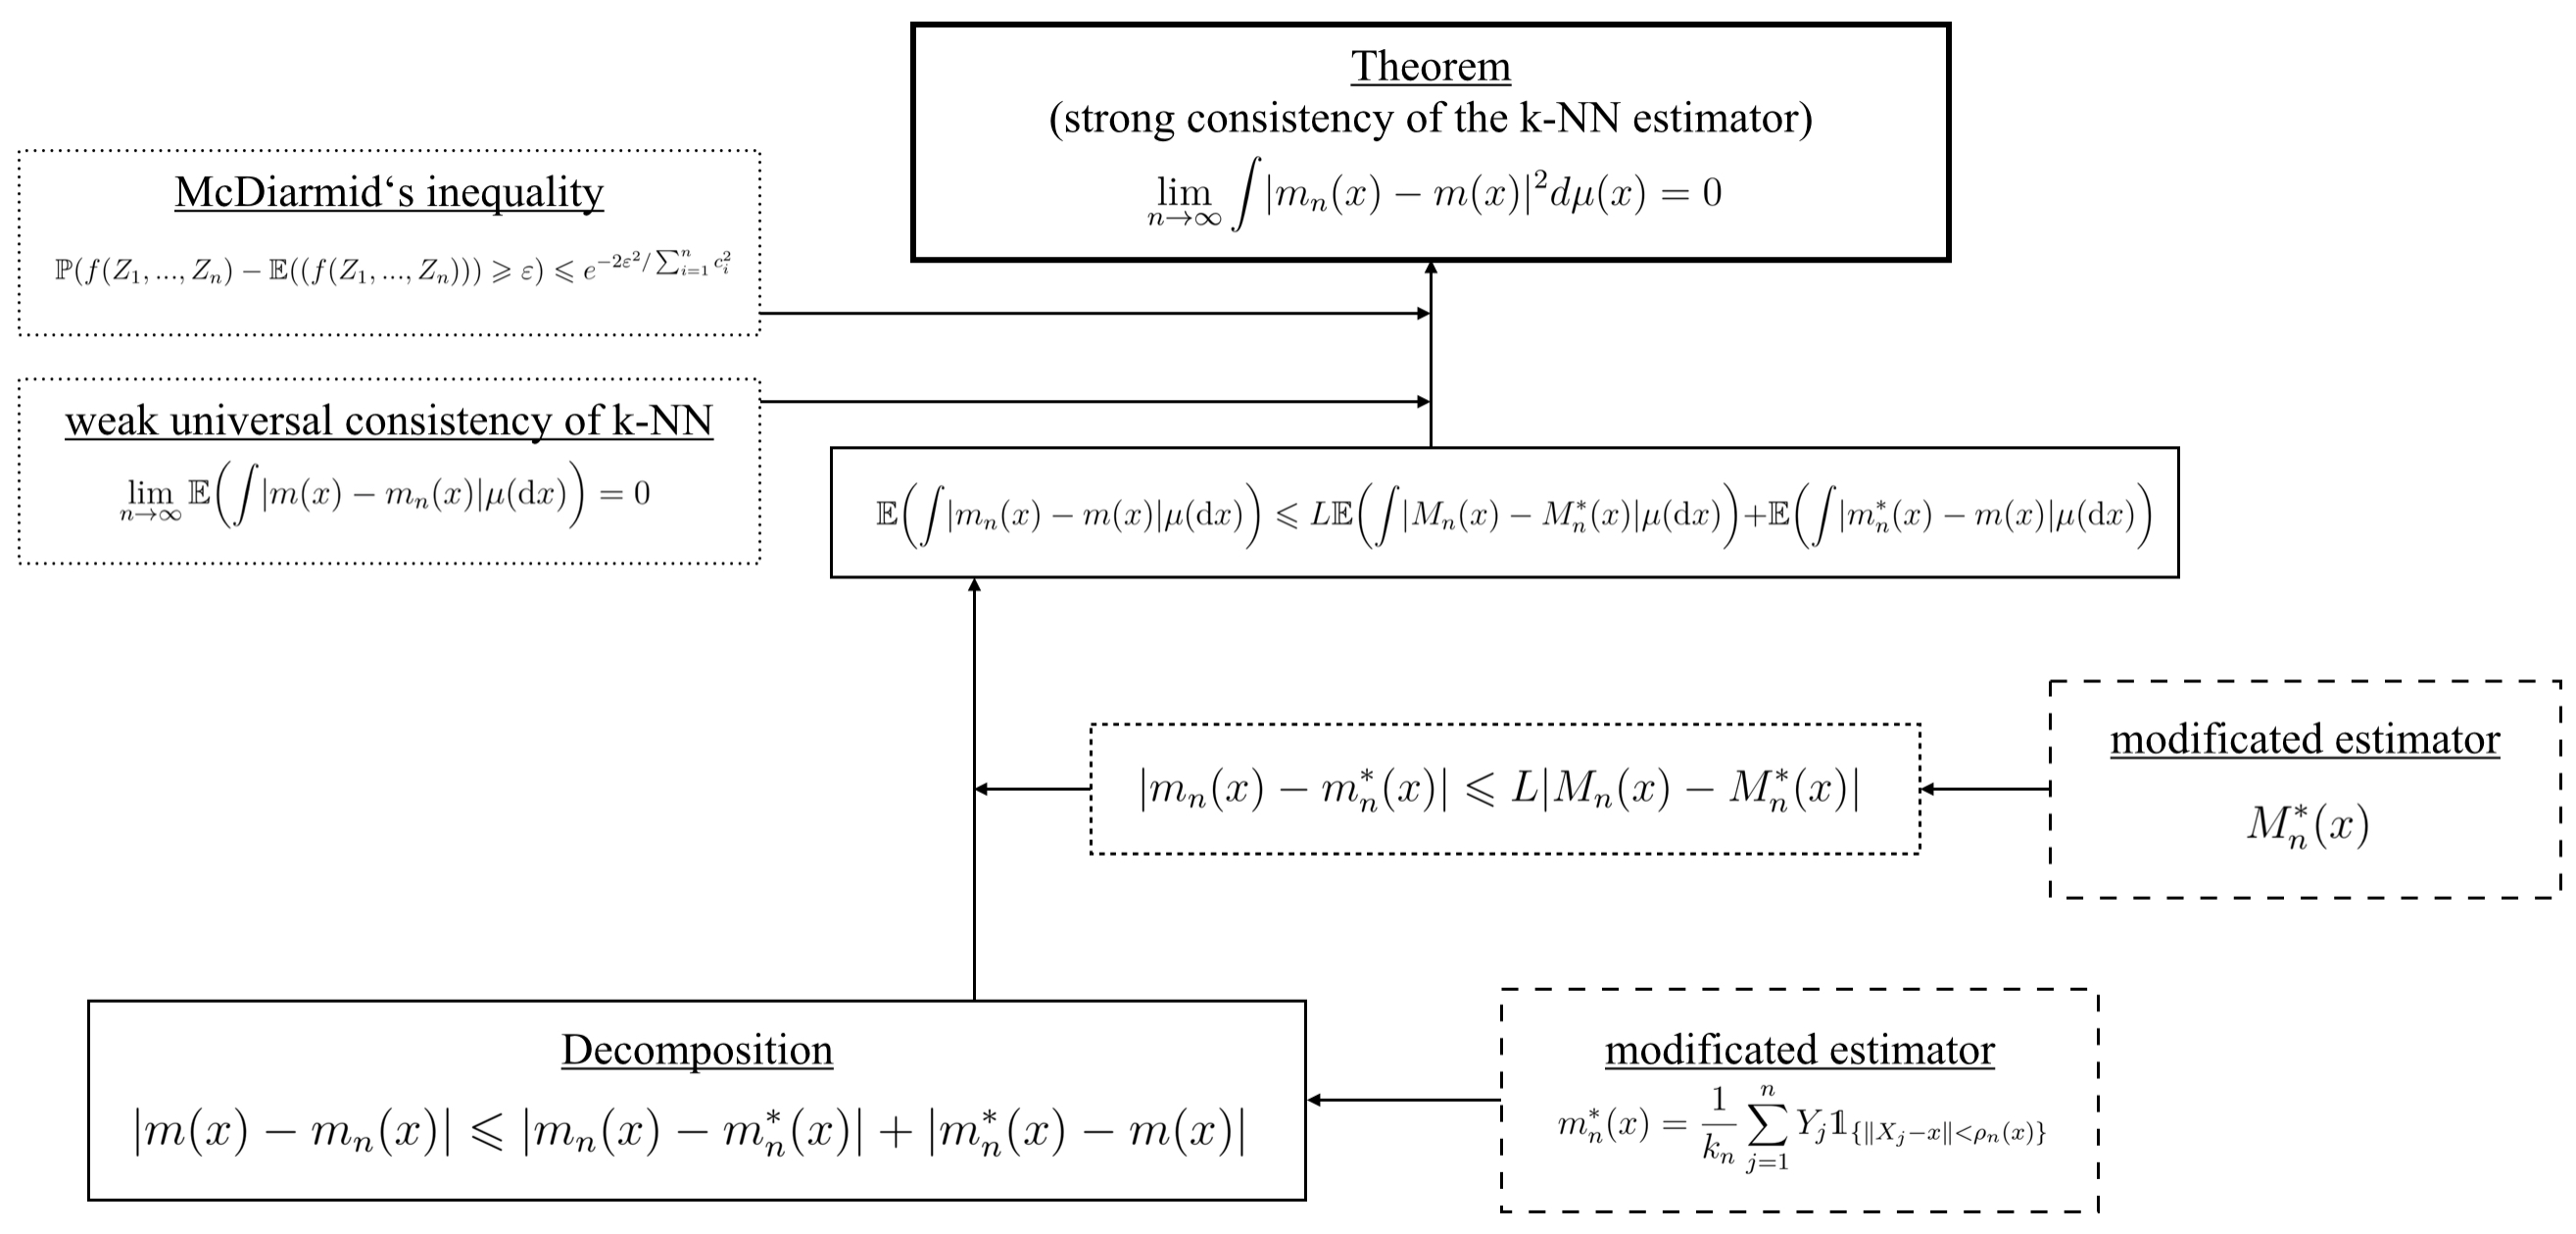
\includegraphics[scale=0.15]{organigramknn.jpeg}
    \centering
    \caption{Organizational chart of the proof of theorem \ref{knnsc}.}
\end{figure}


\begin{proof}
    We first show that, for sufficiently large \(n\)
    \[
        \pro{\int \abs{m(x) - m_n(x)} \mu(\dx) > \epsilon}
        \leq 4e^{-n\epsilon^2 / (72 L^2 \gamma^2_d)}
    \]
    where we defined \(\gamma_d\) as in \nameref{lemma6.2} (see the Appendix). Due to \(\norm{X - x}\) being absolutely continuous. (note that this is the only part in the proof where we will make use of this assumption), we know by Radon-Nikodým's Theorem \ref{radonnikodym} and its corollary \ref{radonnikodymcorollary}, that \(\norm{X - x}\) has a probability density function (PDF) \(f_{\norm{X - x}}\). We now define \(\varrho_n(x)\) for every \(x \in \R^d\) and \(n \in \N\) as the solution to the equation
    \[
        \frac{k_n}{n} = \mu(B_{\varrho_n(x)}(x)) = P(\norm{X - x} < \varrho_n(x)) = \int_{-\infty}^{\varrho_n(x)} f_{\norm{X - x}}(t) \dt
    \]
    and \(\varrho_n(x)\) is well-defined.
    Also define \(m_n^*(x)\) by
    \[
        m_n^*(x) = \frac{1}{k_n}\sum_{j=1}^n Y_j \ind{\{\norm{X_j - x} < \varrho_n(x)\}}.
    \]
    For the proof we will rely on the following decomposition:
    \[
        \abs{m(x) - m_n(x)} \leq \abs{m_n(x) - m_n^*(x)} + \abs{m_n^*(x) - m(x)}.
    \]
    By denoting \(R_n(x) := \norm{X_{(k_n, n)}(x) - x}\), we see that
    \begin{align*}
        \abs{m_n^*(x) - m_n(x)}
        &= \frac{1}{k_n}\abs[\Bigg]{\sum_{j=1}^n Y_j \ind{\{X_j \in B_{\varrho_n(x)}(x)\}} - \sum_{j=1}^n Y_j \ind{\{X_j \in B_{R_n(x)}(x)\}}} \\
        &\leq \frac{L}{k_n} \sum_{j=1}^n\abs[\big]{ \ind{\{X_j \in B_{\varrho_n(x)}(x)\}} - \ind{\{X_j \in B_{R_n(x)}(x)\}}}. \quad (\abs{Y} \leq L \ \text{a.s.})
    \end{align*}
    For fixed \(x\) we have either \(\varrho_n(x) \leq R_n(x)\) or \(\varrho_n(x) \geq R_n(x)\), thus either \(B_{\varrho_n(x)}(x) \subseteq B_{R_n(x)}(x)\) or \(B_{\varrho_n(x)}(x) \supseteq B_{R_n(x)}(x)\) and therefore
    \(\ind{\{X_j \in B_{\varrho_n(x)}(x)\}} - \ind{\{X_j \in B_{R_n(x)}(x)\}}\) have the same sign for each \(j\). It follows that
    \begin{align*}
        \abs{m_n^*(x) - m_n(x)}
        &\leq \frac{L}{k_n} \sum_{j=1}^n\abs[\big]{ \ind{\{X_j \in B_{\varrho_n(x)}(x)\}} - \ind{\{X_j \in B_{R_n(x)}(x)\}}} \\
        &= L \abs[\Bigg]{\frac{1}{k_n} \sum_{j=1}^n (\ind{\{X_j \in B_{\varrho_n(x)}(x)\}} - \ind{\{X_j \in B_{R_n(x)}(x)\}})} \\
        &= L \abs[\Bigg]{\frac{1}{k_n} \sum_{j=1}^n \ind{\{X_j \in B_{\varrho_n(x)}(x)\}} - \frac{k_n}{k_n}} \quad \text{(by definition of \(R_n(x)\))}\\
        &= L \abs[\Bigg]{\frac{1}{k_n} \sum_{j=1}^n \ind{\{X_j \in B_{\varrho_n(x)}(x)\}} - 1} \\
        &= L\abs{M_n^*(x) - M(x)}
    \end{align*}
    where \(M_n^*\) is defined as \(m_n^*\) with Y replaced by the constant random variable \(Y \equiv 1\), and \(M \equiv 1\) is the corresponding regression function.
    We note that
    \begin{align*}
        \ev{M_n^*(x)}
        &= \ev{\frac{1}{k_n}\sum_{j=1}^n \ind{\{X_j \in B_{\varrho_n(x)}(x)\}}} \\
        &= \frac{1}{k_n} \sum_{j=1}^n \pro{X_j \in B_{\varrho_n(x)}(x)} \\
        &= \frac{1}{k_n} \sum_{j=1}^n \mu(B_{\varrho_n(x)}(x)) \\
        &= \frac{1}{k_n} \sum_{j=1}^n \frac{k_n}{n} \quad (\text{by the definition of} \ \varrho(x))\\
        &= 1 \\
        &= M(x)
    \end{align*}
    So far, we've got
    \begin{equation} \label{knnscfirsteq}
        \abs{m(x) - m_n(x)} \leq L\abs{M_n^*(x) - M(x)} + \abs{m_n^*(x) - m(x)}.
    \end{equation}
    First we show that the expected values of the integrals of both terms on
    the right-hand side converge to zero. Then we use McDiarmid’s inequality
    to prove that both terms are very close to their expected values with large
    probability.
    For the expected value of the first term on the right-hand side of
    (\ref{knnscfirsteq}), we have
    \begin{align*}
        &\quad \ L\ev{\int \abs{M_n^*(x) - M(x)} \mu(\dx)} \\
        &= L \int \ev{\abs{M_n^*(x) - M(x)}} \mu(\dx) \quad \text{(Fubini)}\\
        &\leq L \int \sqrt{\ev{\abs{M_n^*(x) - M(x)}^2}} \mu(\dx) \quad \text{(Cauchy-Schwarz inequality)} \\
        &= L \int \sqrt{\ev{\abs{M_n^*(x) - \ev{M_n^*(x)}}^2}} \mu(\dx) \quad \text{(equation from above)} \\
        &= L \int \sqrt{\var{M_n^*(x)}} \mu(\dx) \\
        &= L \int \sqrt{\frac{1}{k_n^2}n\var{\ind{\{X \in B_{\varrho_n(x)}(x)\}}}} \mu(\dx) \quad (X, X_1, \ldots, X_n \ \text{iid.})\\
        &\leq L \int \sqrt{\frac{1}{k_n^2}n\ev{\ind{\{X \in B_{\varrho_n(x)}(x)\}}^2}} \mu(\dx) \\
        &= L \int \sqrt{\frac{1}{k_n^2}n\pro{X \in B_{\varrho_n(x)}(x)}} \mu(\dx) \\
        &= L \int \sqrt{\frac{1}{k_n^2}n\mu(B_{\varrho_n(x)}(x))} \mu(\dx)  \\
        &= L \int \sqrt{\frac{n}{k_n^2} \frac{k_n}{n}} \mu(\dx) \quad \text{(definition of \(\varrho_n(x)\))} \\
        &= \frac{L}{\sqrt{k_n}},
    \end{align*}
    which converges to \(0\) for \(n \to \infty\). For the expected value of the second term on the right-hand side of (\ref{knnscfirsteq}), we use the weak universal consistency of the $k$-NN Estimator:
    \[
        \limn \ev{\int \abs{m(x) - m_n(x)} \mu(\dx)} = 0.
    \]
    Therefore,
    \begin{align} \label{knnmodifiedconvergence}
        &\ev{\int \abs{m_n^*(x) - m(x)} \mu(\dx)} \\
        &\leq \ev{\int \abs{m_n^*(x) - m_n(x)} \mu(\dx)} + \ev{\int \abs{m(x)- m_n(x)} \mu(\dx)} \nonumber \\
        &\leq L \ev{\int \abs{M_n^*(x) - M_n(x)} \mu(\dx)} + \ev{\int \abs{m(x)- m_n(x)} \mu(\dx)} \nonumber \\
        &\longrightarrow 0 \nonumber.
    \end{align}
    % Thus, for all \(\epsilon > 0\) there exists \(n\) sufficiently large enough, such that
    % \[
    %     L \ev{\int \abs{M_n^*(x) - M_n(x)} \mu(\dx)} + \ev{\int \abs{m(x)- m_n(x)} % \mu(\dx)} < \frac{\epsilon}{3}.
    % \]
    We notice that for random Variables A, B, C,
    \begin{align} \label{probeq2}
        \pro{A + B > 2C} \leq \pro{A > C} + \pro{B > C}.
    \end{align}
   
    Assume now by (\ref{knnmodifiedconvergence}) that \(n\) is so large that
    \[
        I_n + J_n := L\ev{\int \abs{M_n^*(x) - M(x)} \mu(\dx)} + \ev{\int \abs{m_n^*(x) - m(x)} \mu(\dx)} < \frac{\epsilon}{3}.
    \]
    Then, with (\ref{knnscfirsteq}), we have for all \(\epsilon > 0\)
    \begin{align}
        &\quad \ \pro{\int \abs{m(x) - m_n(x)} \mu(\dx) > \epsilon} \\
        &= \pro{\int \abs{m(x) - m_n(x)} \mu(\dx) - I_n - J_n > \epsilon - I_n - J_n} \nonumber \\
        &\leq \pro{\int \abs{m(x) - m_n(x)} \mu(\dx) - I_n - J_n > 2\frac{\epsilon}{3}} \quad \text{(by (\ref{probeq1}))}\nonumber \\
        &\leq \pro{\int L\abs{M_n^*(x) - M(x)} \mu(\dx) + \int \abs{m_n^*(x) - m(x)} \mu(\dx) - I_n - J_n > 2\frac{\epsilon}{3}} \quad \text{(by (\ref{probeq1}))} \nonumber \\
        &\leq \pro{\int \abs{m_n^*(x) - m(x)} \mu(\dx) - I_n  > \frac{\epsilon}{3}} \nonumber  \\
        &+ \pro{L\int \abs{M_n^*(x) - M(x)} \mu(\dx) - J_n > \frac{\epsilon}{3}} \quad \text{(by (\ref{probeq2}))}\nonumber \\
        &= \pro{\int \abs{m_n^*(x) - m(x)} \mu(\dx) - \ev{\int \abs{m_n^*(x) - m(x)} \mu(\dx)}  > \frac{\epsilon}{3}} \nonumber \\
        &+ \pro{L\int \abs{M_n^*(x) - M(x)} \mu(\dx) - \ev{L\int \abs{M_n^*(x) - M(x)} \mu(\dx)}  > \frac{\epsilon}{3}}  \nonumber.
    \end{align}
    %% P(a + b > 2c) <= P(a > c) + P(b > c)

    Next we get an exponential bound for the first probability on the right-hand
    side of (\ref{knnscfirsteq}) by McDiarmid's inequality. We fix an arbitrary realization of the data \(D_n = \{(x_1, y_1), \ldots, (x_n, y_n)\}\), and replace \((x_i, y_i)\) by \((\hat{x_i}, \hat{y_i})\), changing the value of \(m_n^*(x)\) to \(m_{ni}^*(x)\). Then by the inverse triangle inequality
    \begin{align*}
        &\quad \ \abs[\bigg]{\int \abs{m_n^*(x) - m(x)} \mu(\dx) - \int \abs{m_{ni}^*(x) - m(x)} \mu(\dx)} \\
        &\leq \int \abs{m_n^*(x) - m_{ni}^*(x)} \mu(\dx) \\
        &= \int \abs[\Big]{\frac{1}{k_n}\left(\sum_{j = 1}^n y_j \ind{\{\norm{x_j - x} < \varrho_n(x)\}} - \hat{y}_i \ind{\{\norm{\hat{x}_i - x} < \varrho_n(x)\}} - \sum_{j \neq 1}^n y_j \ind{\{\norm{x_j - x} < \varrho_n(x)\}}\right)} \mu(\dx) \\
        &= \frac{1}{k_n} \int \abs{y_i \ind{\{\norm{x_i - x} < \varrho_n(x)\}} - \hat{y}_i \ind{\{\norm{\hat{x}_i - x} < \varrho_n(x)\}}} \mu(\dx)
    \end{align*}
    But \(\abs{y_i \ind{\{\norm{x_i - x} < \varrho_n(x)\}} - \hat{y}_i \ind{\{\norm{\hat{x}_i - x} < \varrho_n(x)\}}}\) is bounded by \(2L\) and can differ from zero only if \(\norm{x - x_i} < \varrho_n(x)\) or \(\norm{x - \hat{x_i}} < \varrho_n(x)\). Observe that \(\norm{x - x_i} < \varrho_n(x)\) or \(\norm{x - \hat{x_i}} < \varrho_n(x)\) if and only if \(\mu(B_{\norm{x - x_i}}(x)) < k_n / n\) due to the definition of \(\varrho_n(x)\). But the measure of such \(x\)'s is bounded by \(2 \cdot \gamma_d k_n / n\) by \nameref{lemma6.2}.
    Therefore,
    \[
        \sup_{x_1, y_1, \ldots, x_n, y_n, \hat{x_i}, \hat{y_i}}
        \int \abs{m_{n}^*(x) - m_{ni}^*(x)} \mu(\dx)
        \leq \frac{2L}{k_n} \frac{2 \cdot \gamma_d k_n}{n} = \frac{4L \gamma_d}{n}
    \]
    and by McDiarmid's inequality \ref{mcdiarmidineq}
    \begin{align*}
        &\quad \ \pro{\int \abs{m_n^*(x) - m(x)} \mu(\dx) - \ev{\int \abs{m_n^*(x) - m(x)} \mu(\dx)}  > \frac{\epsilon}{3}} \\
        &\leq 2e^{-n\epsilon^2 / (72L^2 \gamma_d^2)}.
    \end{align*}
    For the second term on the right-hand side of (\ref{knnscfirsteq}), we can do it in exactly the same way, yielding
    \begin{align*}
        &\quad \ \pro{L\int \abs{M_n^*(x) - M(x)} \mu(\dx) - \ev{L\int \abs{M_n^*(x) - M(x)} \mu(\dx)}  > \frac{\epsilon}{3}} \\
        &\leq 2e^{-n\epsilon^2 / (72L^2 \gamma_d^2)}.
    \end{align*}
    Putting that into (\ref{knnscfirsteq}) gives us
    \[
        \pro{\int \abs{m(x) - m_n(x)} \mu(\dx) > \epsilon}
        \leq 4e^{-n\epsilon^2 / (72 L^2 \gamma^2_d)}.
    \]
    Thus by the Borel-Cantelli Lemma, we get for every \(\epsilon > 0\) that
    \[
        \limsup_{n \to \infty} \int \abs{m(x) - m_n(x)} \mu(\dx) < \epsilon \ \text{almost surely}.
    \]
   
    Due to the $k$-NN estimate having probability weights, we get
    \[
        \abs{m(x) - m_n(x)} \leq \abs{m(x)} + \abs{m_n(x)} \leq 2L
    \]
    almost surely.
    Therefore finally
    \begin{align*}
        \lim_{n \to \infty} \int \abs{m(x) - m_n(x)}^2 \mu(\dx)
        \leq \lim_{n \to \infty} 2L\int \abs{m(x) - m_n(x)} \mu(\dx)
        = 0
    \end{align*}
    almost surely because \(\epsilon\) was chosen arbitrarily small.
   
    
    
\end{proof}

Before we come to the formulation and proof of the theorem for strong universal consistency of the $k$-NN estimate, we first of all need to show two lemmata. We now define some useful sets that we will continue to use in the course of our proof.

\begin{definition} \label{knnai}
    Let \(A_i\) be the collection of all \(x \in \R^d\) s.t.\@ \(X_i\) is one of its \(k_n\) nearest neighbors of \(x\) in \(\{X_1, \ldots, X_n\}\).
\end{definition}

 Let us define cones \(x + C_1, \ldots, x + C_{\gamma_d}\) as we did in Lemma 6.2. where 
\begin{align*}
    \bigcup_{j=1}^{\gamma_d} C_j = \R^d.
\end{align*}
Then obviously
\begin{align} \label{cover}
    \bigcup_{j=1}^{\gamma_d} \{x + C_j\} = \R^d
\end{align}
regardless of how we chose \(x\). By the cone property, if \(u, u' \in x + C_j\) and \(\norm{x - u} < \norm{x - u'}\), then \(\norm{u - u'} < \norm{x - u'}\). Define
\[
    C_{i, j} = X_i + C_j \quad 1 \leq i \leq n, 1 \leq j \leq \gamma_d.
\]

\begin{definition} \label{knnbi}
    Let \(B_{i, j}\) be the subset of \(C_{i, j}\) consisting of all \(x \in C_{i, j}\) that are among the \(k_n\) nearest neighbors of \(X_i\) in the set
    \[
        \{X_1, \ldots, X_{i-1},X_{i+1}, \ldots, X_n, x\} \cap C_{i, j}. 
    \]
    (If \(C_{i, j}\) contains fewer than \(k_n-1\) of the \(X_l\) points \(i \neq l\), then \(B_{i, j} = C_{i, j}\).) Equivalently \(B_{i, j}\) is the subset of \(C_{i, j}\) consisting of all \(x\) that are closer to \(X_i\) than the \(k_n\)-th nearest neighbor of \(X_i\) in \(\{X_1, \ldots, X_{i-1}, X_{i+1}, \ldots, X_n\} \cap C_{i, j}\).
    
\end{definition}

\begin{lemma}[$k$-NN covering] \label{knncoverlemma}
Let \(1 \leq i \leq n\). If \(x \in A_i\), then \(x \in \bigcup_{j=1}^{\gamma_d} B_{i,j}\), and thus
\[
    \mu(A_i) \leq \sum_{j=1}^{\gamma_d}\mu(B_{i,j}).
\]
where \(A_i\) and \(B_{i,j}\) are defined as in Definition \ref{knnai} and \ref{knnbi} respectively.
\end{lemma}

\begin{proof}
    Take \(x \in A_i\). Then locate a \(j\) for which \(x \in C_{i,j}\) (this always exists because of (\ref{cover})). We now have to show, that \(x \in B_{i, j}\) and the claim is proven. Equivalently, \(x\) has to be one of the \(k_n\) nearest neighbors of \(X_i\) in the set
    \[
        \{X_1, \ldots, X_{i-1},X_{i+1}, \ldots, X_n, x\} \cap C_{i, j}. 
    \]
    Take \(X_l \in C_{i,j}\). If \(\norm{X_l - X_i} < \norm{x - X_i}\), then by the cone property we get that \(\norm{x - X_l} < \norm{x - X_i}\), and thus \(X_l\) is one of the \(k_n - 1\) nearest neighbors of \(x\) in \(\{X_1, \ldots, X_n\}\) because of \(x \in A_i\) (by definition of \(A_i\), \(X_l\) being the \(k_n\)-th nearest neighbor of \(x\) in \(\{X_1, \ldots, X_n\}\) would already imply \(l = i\)). This shows that in \(C_{i,j}\) there are most \(k_n - 1\) points \(X_l\) closer to \(X_i\) than \(x\). Thus \(x\) is one of the \(k_n\) nearest neighbors of \(X_i\) in the set
    \[
        \{X_1, \ldots, X_{i-1},X_{i+1}, \ldots, X_n, x\} \cap C_{i, j}.
    \]
    This concludes the proof of the claim.
\end{proof}


\begin{lemma}[$k$-NN upper bound for \(\mu(B_{i, j})\) as \(n \to \infty\)] \label{knnlemmatwo}
Assume that for each x the random variable \(\norm{X - x}\) is absolutely continuous.
If \(k_n / \log(n) \to \infty\) and \(k_n / n \to 0\) then, for every  \(j \in \{1, \ldots, \gamma_d\}\),

\[
    \limsup_{n \to \infty} \frac{n}{k_n}\max_{1 \leq i \leq n} \mu(B_{i, j}) \leq 2 \ a.s.,
\]
where \(B_{i,j}\) are defined as in Definition \ref{knnbi}.
\end{lemma}

\begin{proof}
    If we utilize the Borel-Cantelli Lemma, we need to show for every \(j\), that
    \[
        \sum_{n=1}^\infty \pro{\frac{n}{k_n}\max_{1 \leq i \leq n} \mu(B_{i, j}) > 2} < \infty
    \]
    In order to do this we give a bound for
    \[
        \pro{\mu(B_{i,j}) > p \mid X_i}
    \]
    for arbitrary \(0 < p < 1\). If \(\mu(C_{i, j}) \leq p\) then since \(B_{i, j} \subseteq C_{i, j}\), we have \(\pro{\mu(B_{i,j}) > p \mid X_i} = 0\), therefore we can assume that \(\mu(C_{i, j}) > p\). Fix \(X_i\). Define
    \[
        G_{i, p} := C_{i, j} \cap B_{R_n(X_i)}(X_i),
    \]
    where \(R_n(X_i) > 0\) is chosen such that \(\mu(G_{i, p}) = p\) (Its existence is assured similar to the proof of Theorem \ref{knnsc}). We notice that either
    \(B_{i, j} \supseteq G_{i, p}\) or \(B_{i, j} \subseteq G_{i, p}\), therefore we have the following relationship:
    \begin{align*}
        &\quad \ \pro{\mu(B_{i, j}) > p \mid X_i} \\
        &= \pro{\mu(B_{i, j}) > \mu(G_{i, p}) \mid X_i} \\
        &= \pro{B_{i, j} \supset G_{i, p} \mid X_i} \\
        &= \pro{\text{\(G_{i, p}\) captures \(< k_n\) of the points} \ X_l \in C_{i, j}, l \neq i \mid X_i} \\
        &= \pro{\sum_{\substack{l = 1 \\ l \neq i}}^n \ind{\{X_l \in G_{i, p}\}} < k_n \Biggm| X_i}
    \end{align*}

    %%%%%%%%

    The number of points \(X_l\) \((l \neq i)\) captured by \(G_{i, p}\) given \(X_i\) is binomially distributed with parameters \((n-1, p)\), so by Lemma A.1, with \(p = 2k_n / (n-1)\) and \(\epsilon = p/2 = k_n/(n-1)\) (which we can both WLOG assume to be smaller than \(1\) due to \(k_n / n \to 0\)), we have that
    \begin{align*}
        &\quad \ \pro{\max_{1 \leq i \leq n} \mu(B_{i,j}) > p} \\
        &= \pro{\cup_{i = 1}^n \{\mu(B_{i,j}) > p\}} \\
        &\leq n \pro{\mu(B_{1, j}) > p} \\
        &= n \ev{\pro{\mu(B_{1, j}) > p \mid X_1}} \\
        &= n \ev{\pro{\text{\(G_{1, p}\) captures \(< k_n\) of the points} \ X_l \in C_{1, j}, l \neq 1 \mid X_1}} \\
        &=  n \ev{\pro{\sum_{\substack{l = 1 \\ l \neq 1}}^n \ind{\{X_l \in G_{1, p}\}} < k_n \Biggm| X_1}} \\
        &=  n \ev{\pro{\sum_{\substack{l = 1 \\ l \neq 1}}^n \ind{\{X_l \in G_{1, p}\}} < (n-1)\frac{k_n}{n-1} \Biggm| X_1}} \\
        &=  n \ev{\pro{\sum_{\substack{l = 1 \\ l \neq 1}}^n \ind{\{X_l \in G_{1, p}\}} < (n-1)\epsilon \Biggm| X_1}} \\
        &\leq ne^{-(n-1)[p-\epsilon+\epsilon \log(\epsilon/p)]} \quad(\text{by Chernoff's inequality \ref{chernoff}}) \\
        &= ne^{-2k_n + k_n + k_n \log 2} \\
        &\leq ne^{-k_n( 1 - \log 2)},
    \end{align*}
    which is summable because \(k_n / \log n \to \infty\) implies there exists \(N \in \N\) s.t.\@ for all \(n \geq N\), we have \(k_n \geq \frac{3}{1-\log 2} \log n\), and thus
    \begin{align*}
        &\quad \ \sum_{n=1}^\infty ne^{-k_n( 1 - \log 2)} \\
        &= \sum_{n=1}^N ne^{-k_n( 1 - \log 2)} + \sum_{n=N+1}^\infty ne^{-k_n( 1 - \log 2)} \\
        &\leq \sum_{n=1}^N ne^{-k_n( 1 - \log 2)} + \sum_{n=N+1}^\infty ne^{-\frac{3}{1-\log 2} \log(n) ( 1 - \log 2)} \\
        &= \sum_{n=1}^N ne^{-k_n( 1 - \log 2)} + \sum_{n=N+1}^\infty n \frac{1}{n^3} \\
        &= \underset{< \infty}{\underbrace{\sum_{n=1}^N ne^{-k_n( 1 - \log 2)}}} + \underset{< \infty}{\underbrace{\sum_{n=N+1}^\infty \frac{1}{n^2}}} < \infty
    \end{align*}
    
\end{proof}

\begin{theorem} \label{knnsuc}
Assume that for each \(x \in \R^d\) the random variable \(\norm{X - x}\) is absolutely continuous. If \(k_n / \log n \to \infty\) and \(k_n / n \to 0\) then the \(k_n\)-NN regression function estimate is strongly universally consistent, i.e.\@ strongly consistent for all distributions \((X, Y)\) with \(\ev{Y^2} < \infty\).
\end{theorem}

\begin{proof}
    By Lemma \ref{lemma23.3} and Theorem \ref{knnsc} it is enough to prove that there is a constant \(c > 0\),
    \[
        \limsup_{n \to \infty} \sum_{i = 1}^n \int W_{ni}(x) \mu(\dx) Y_i^2 \leq c \ev{Y^2} \quad \text{a.s.}
    \]
    Observe that
    \[
        \sum_{i = 1}^n \int W_{ni}(x) \mu(\dx) Y_i^2 = \frac{1}{k_n} \sum_{i=1}^n Y_i^2 \mu(A_i) \leq \left( \frac{n}{k_n} \max_i \mu(A_i) \right) \frac{1}{n} \sum_{i = 1}^n Y_i^2.
    \]
    If we can show, that
    \begin{equation} \label{eqknnsuc}
        \limsup_{n \to \infty} \frac{n}{k_n} \max_i \mu(A_i) \leq c \quad \text{a.s.}
    \end{equation}

    for some constant \(c > 0\), then by the law of large numbers
    \begin{align*}
        \limsup_{n \to \infty} \left( \frac{n}{k_n} \max_i \mu(A_i) \right) \frac{1}{n} \sum_{i = 1}^n Y_i^2 \leq \limsup_{n \to \infty} c \frac{1}{n} \sum_{i = 1}^n Y_i^2 = c \ev{Y^2} \quad \text{a.s.}
    \end{align*}
    so we need to show (\ref{eqknnsuc}). By the \nameref{knncoverlemma}-Lemma \ref{knncoverlemma}, we have
    \[
        \mu(A_i) \leq \sum_{j=1}^{\gamma_d}\mu(B_{i,j}) \quad \forall i \in \{1, \ldots, n\} 
    \]
    and thus
    \begin{align*}
        &\quad \ \limsup_{n \to \infty} \frac{n}{k_n} \max_i \mu(A_i) \\
        &\leq \limsup_{n \to \infty} \frac{n}{k_n} \max_i \sum_{j=1}^{\gamma_d}\mu(B_{i,j}) \\
        &\leq \limsup_{n \to \infty} \frac{n}{k_n} \sum_{j=1}^{\gamma_d} \max_i \mu(B_{i,j}) \\ 
        &\leq \sum_{j=1}^{\gamma_d} \limsup_{n \to \infty} \frac{n}{k_n}  \max_i \mu(B_{i,j}) \\
        &\leq \sum_{j=1}^{\gamma_d} 2 \quad \text{(by Lemma \ref{knnlemmatwo})} \\
        &= 2 \gamma_d
    \end{align*}
    almost surely.
    
\end{proof}
\newpage

\section{Comparison}
Now, we have been able to fill in the remaining gaps concerning the weak and strong universal consistency of the three estimators. In order to conclude this topic, the two following charts (Figure \ref{comp_kernel}, Figure \ref{comp_knn}) will provide an overview of the prerequisites required to achieve the different types of consistency. Starting for the kernel estimate:

\begin{figure}[h] \label{comp_kernel}
    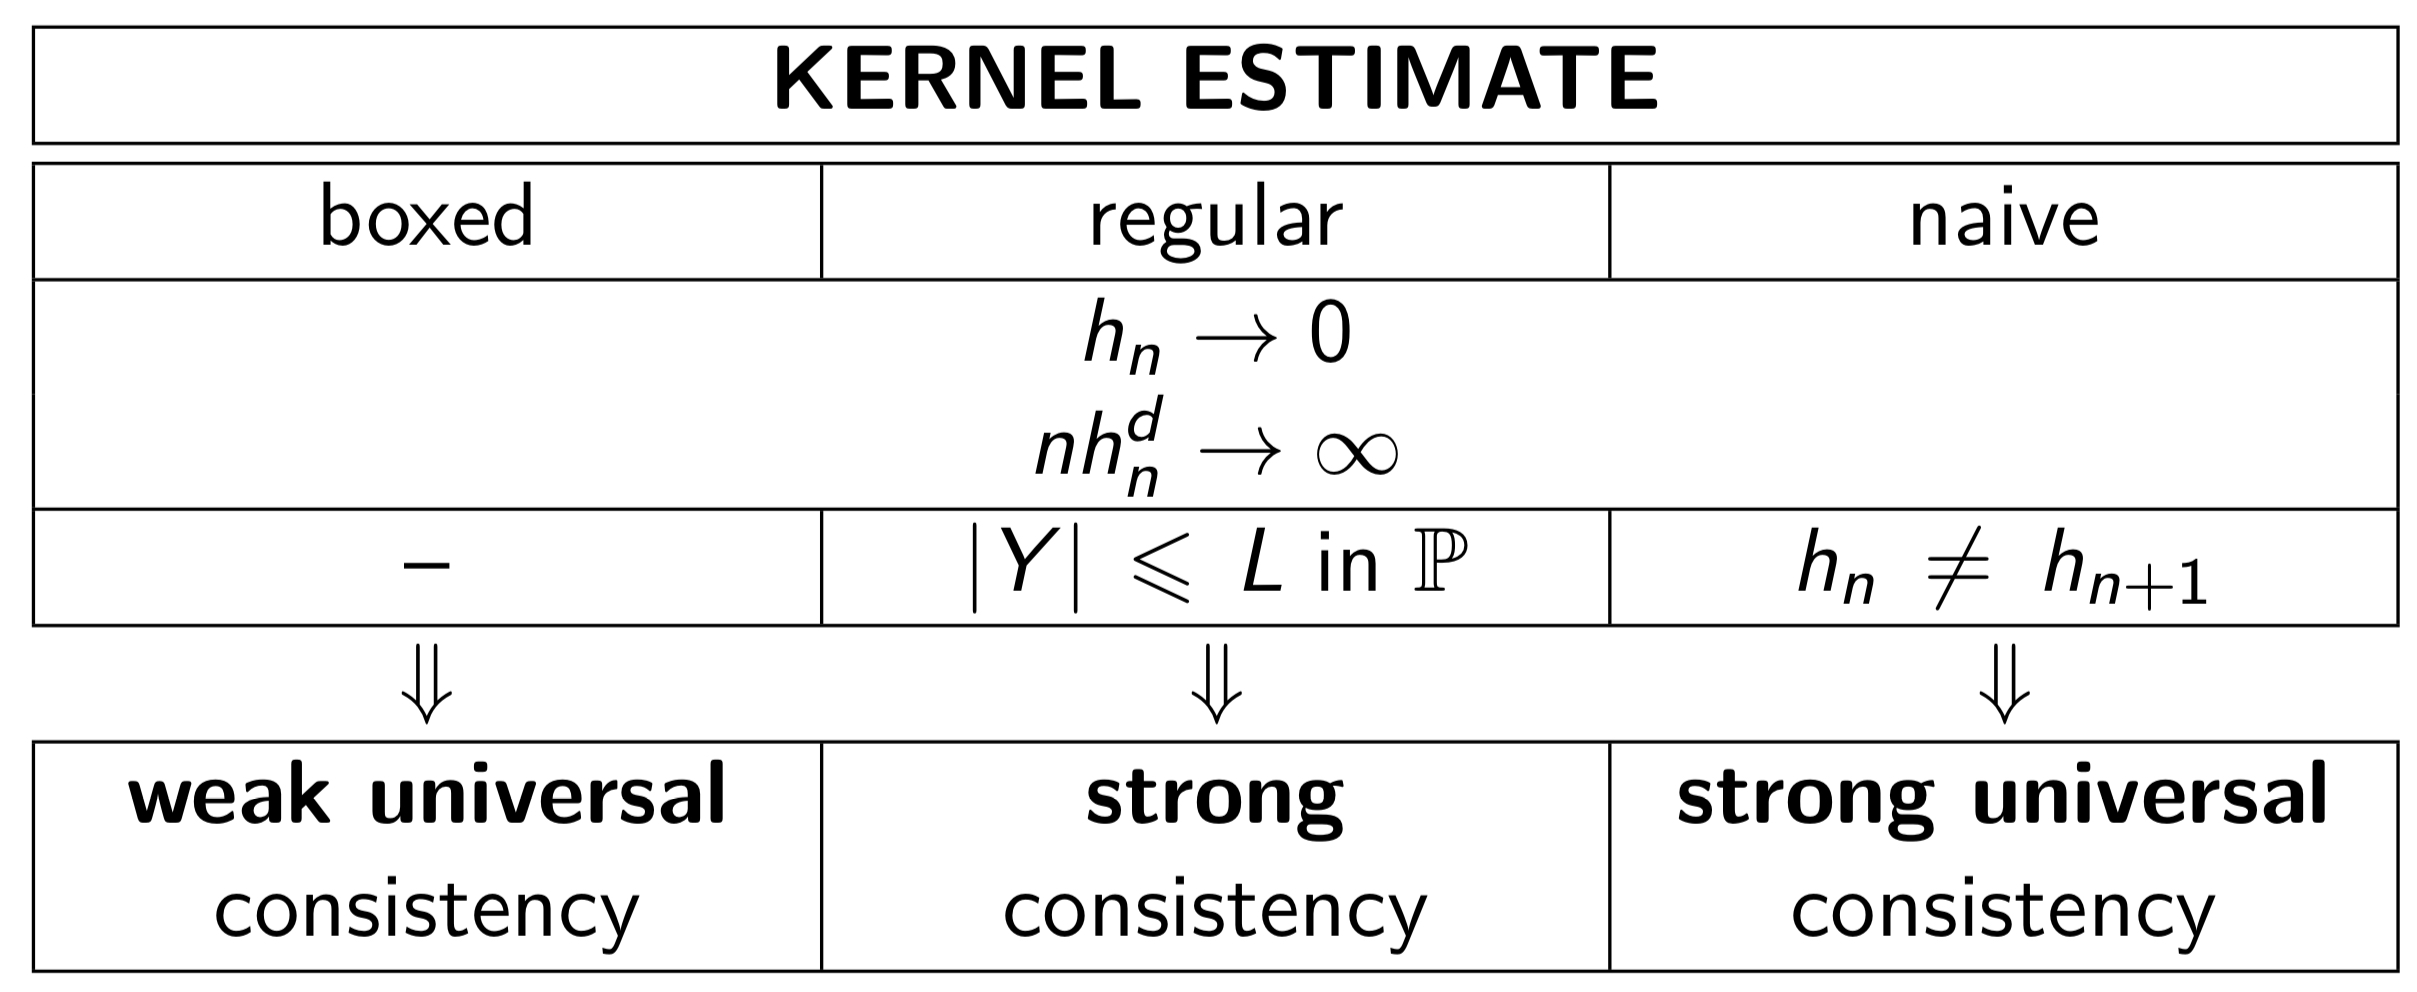
\includegraphics[scale=0.15]{comp_kernel.jpeg}
    \centering
    \caption{Consistencies of kernel estimate (overview).}
\end{figure}

Analogous for the $k$-NN estimate:

\begin{figure}[h] \label{comp_knn}
    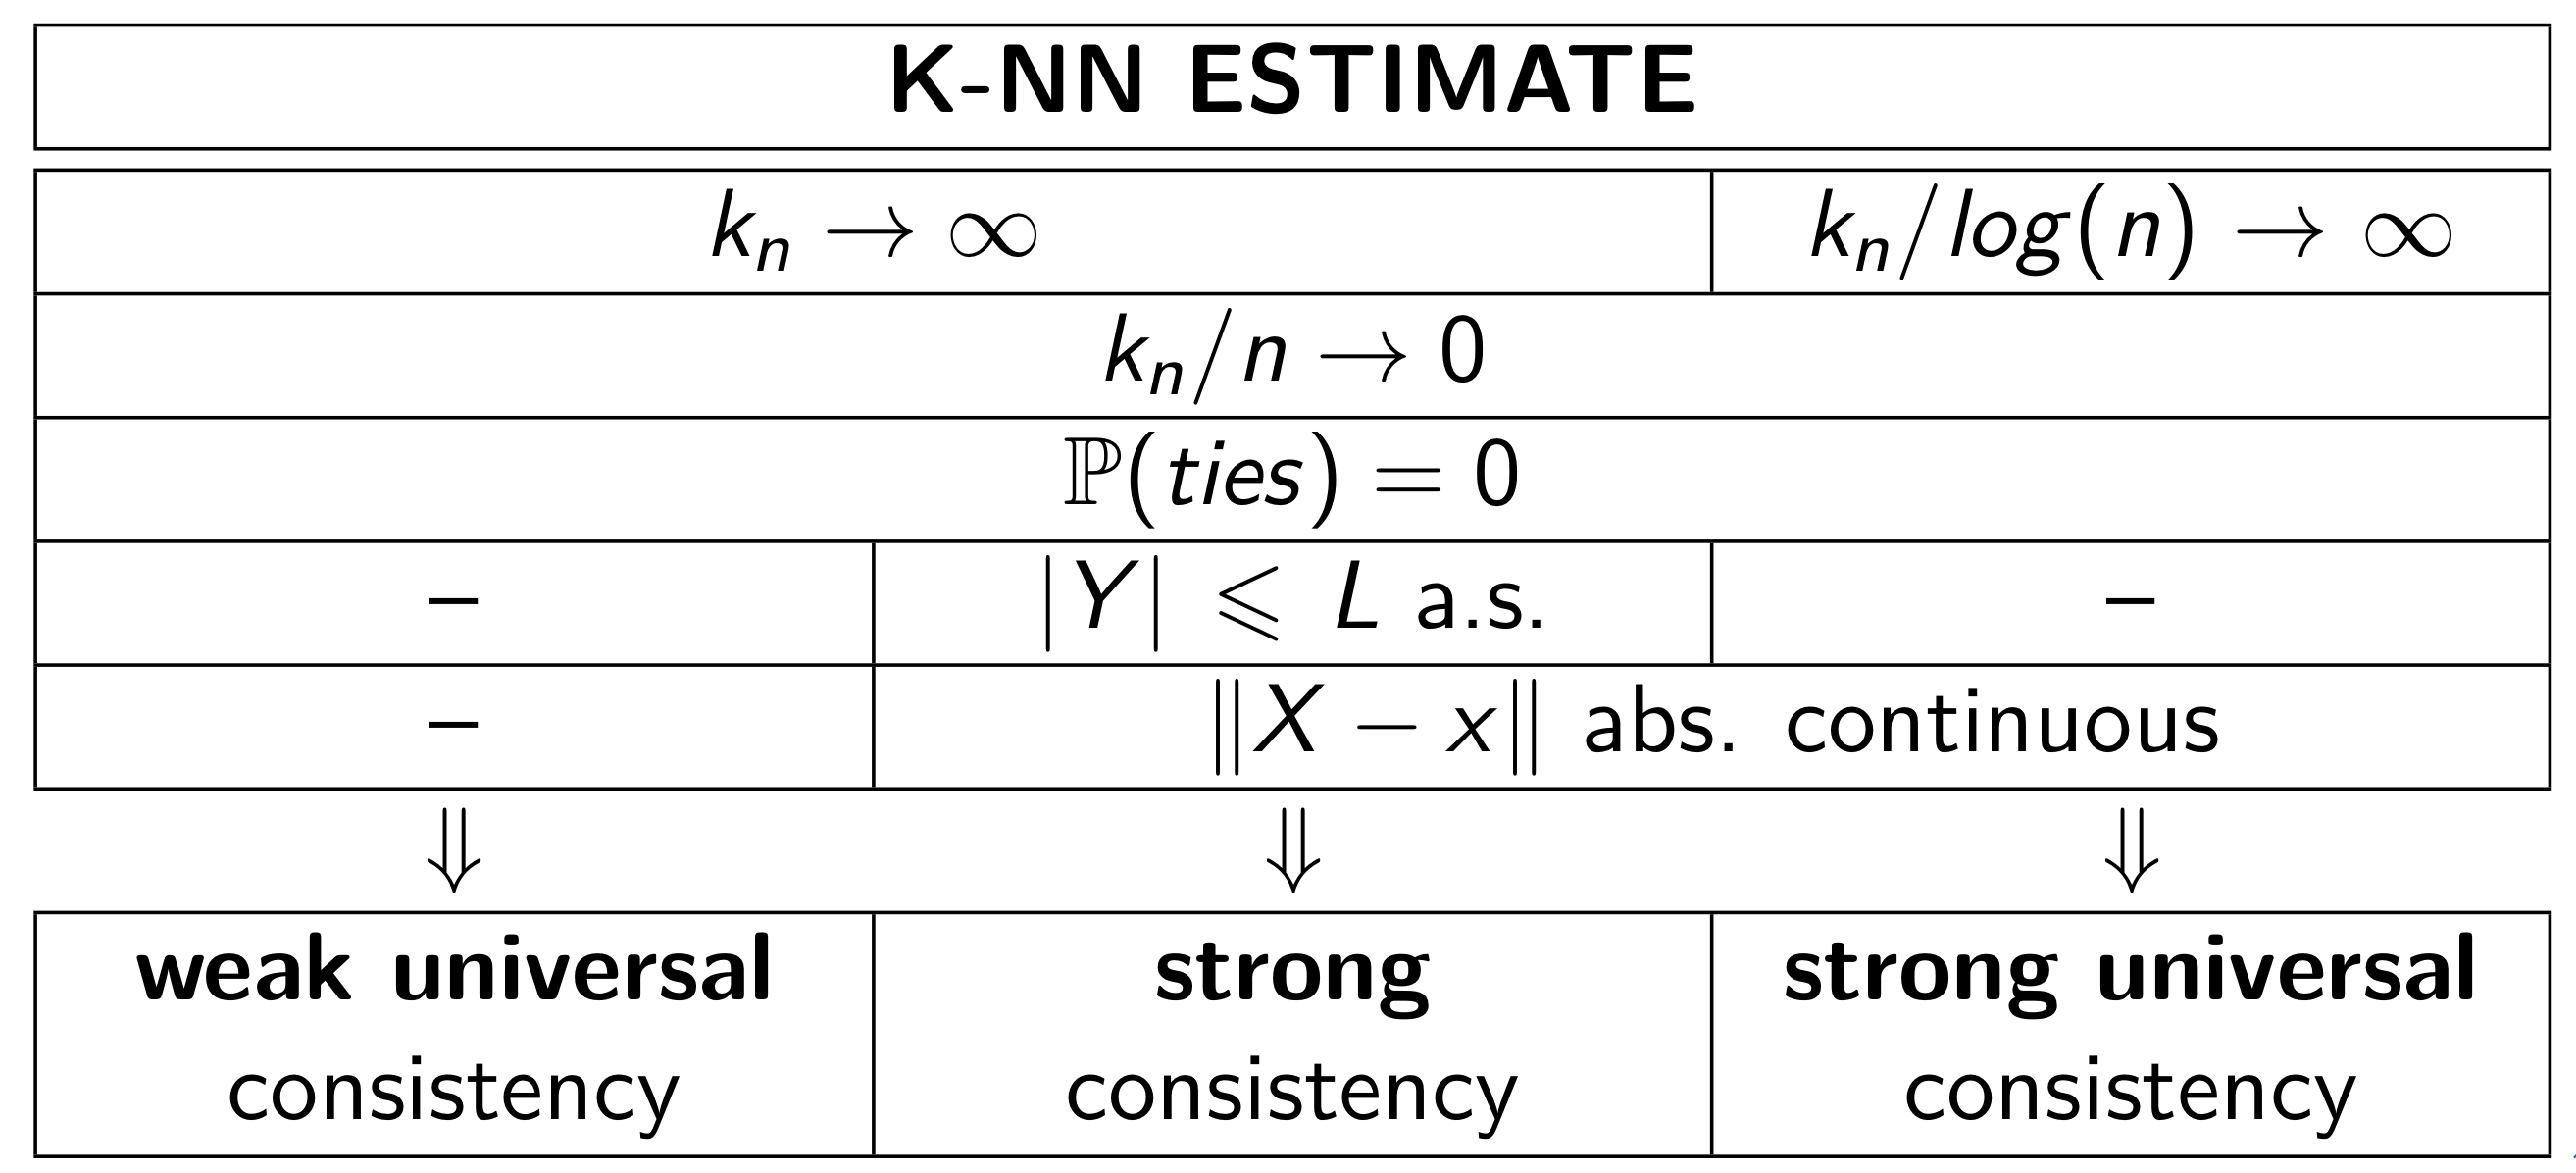
\includegraphics[scale=0.139]{comp_knn.jpeg}
    \centering
    \caption{Consistencies of $k$-NN estimate (overview).}
\end{figure}


\newpage

% Appendix
\appendix
\section{Appendix}

\begin{theorem}[\textsc{Banach-Steinhaus}] \label{banachsteinhaus} % theorem 23.2
 Let $K_n(x,z)$ be functions on $\R^d \times \R^d$ satisfying the following conditions:
\begin{enumerate} [label=(\roman*)]
    \item There is a constant $c>0$ such that, for all $n$,
        \[\int |K_n(x,z)| \mu(\diff{x}) \leq c\]
        for $\mu$-almost all $z$.
    \item There is a constant $D \geq 1$ such that, for all $n$,
        \[\int |K_n(x,z)| \mu(\diff{z}) \leq D\]
        for all $x$.
    \item For all $a>0$,
        \[ \lim\limits_{n \rightarrow \infty} \int \int |K_n(x,z)| \ind{\{ \norm{x-z} > a\}} \mu(\diff{z}) \mu(\diff{x}) = 0. \]
    \item \[ \lim\limits_{n \rightarrow \infty} \text{ess}\sup\limits_{x} | \int K_n(x,z) \mu(\diff{z})     -1 | = 0.\]
\end{enumerate}
Then, for all $m \in L_1(\mu)$,
\[\lim\limits_{n \rightarrow \infty} \int | m(x) - \int K_n(x,z)m(z) \mu(\diff{z}) | \mu(\diff{x}) = 0.\] 
\end{theorem}

\begin{theorem}[\textsc{McDiarmid}] \label{mcdiarmidineq}
    Let $Z_1,...,Z_n$ be independent random variables taking values in a set $A$ and assume that $f:\: A^n \rightarrow \R$ satisfies
    \[
        \sup\limits_{z_1,...,z_n,\hat{z_i} \in A} |f(z_1,...,z_n) - f(z_1,...,z_{i-1},\hat{z_i}, z_{i-1},...,z_n)| \leq c_i, \quad 1 \leq i \leq n.
    \]
    Then, for all $\epsilon > 0$,
    \[
        \pro{f(Z_1,...,Z_n) - \ev{f(Z_1,...,Z_n)} \geq \epsilon} \leq e^{-2\epsilon^2/\sum_{i=1}^n c_i^2}
    \]
    and
    \[
        \pro{\ev{f(Z_1,...,Z_n)} - f(Z_1,...,Z_n) \geq \epsilon} \leq e^{-2\epsilon^2/\sum_{i=1}^n c_i^2}.
    \]
\end{theorem}

\begin{lemma}[\textsc{Györfi}'s Lemma]  \label{lemma6.2}
    \textsc{(Called Lemma 6.2 in Györfi's book)}
    Let
    \[
        \mathcal{B}_a(x') := \{x \in \R^d \mid \mu(B_{\norm{x - x'}}(x)) < a\}.
    \]
    Then, for all \(x' \in \R^d\),
    \[
        \mu(\mathcal{B}_a(x')) \leq \gamma_d a,
    \]
    where \(\gamma_d\) depends on the dimension \(d\) only.
\end{lemma}

\begin{theorem}[\textsc{Radon-Nikodým}] \label{radonnikodym}
Let \(\mu\) and \(\nu\) be measures on \((\Omega, \mathcal{F})\) and let \(\mu\) be \(\sigma\)-finite, the following are equivalent
\begin{enumerate}[a)]
    \item \(\nu\) is continuous with respect to \(\mu\).
    \item There exists a density function \(f \geq 0\), s.t.\@ \(\nu = f\mu\).
\end{enumerate}
\end{theorem}

\begin{corollary} \label{radonnikodymcorollary}
Let \(X\) be an absolutely continuous random variable. Then \(X\) has a PDF.
\end{corollary}

\begin{proof}
    A measure \(\mu\) is absolutely continuous if and only if its measure generating function \(F\), i.e.\@ \(\mu((a, b]) = F(b) - F(a)\), is absolutely continuous. In the case of X, its measure generating function is its CDF and thus \(\mu := \mathbb{P}_X\) is absolutely continuous and by \ref{radonnikodym}, \(X\) has a PDF.
\end{proof}

\begin{lemma}[\textsc{Chernoff}] \label{chernoff}
    Let \(B\) be a binomial random variable with parameters \(n\) and \(p\). Then, for \(1 > \epsilon > p > 0\),
    \[
        \pro{B > n\epsilon}
        \leq \exp\left(-n\left[\epsilon \log \frac{\epsilon}{p} + (1 - \epsilon) \log \frac{1-\epsilon}{1 - p} \right]\right)
        \leq \exp(-n[p-\epsilon+\epsilon \log(\epsilon/p)])
    \]
    and, for \(0 < \epsilon < p < 1\),
    \[
        \pro{B < n\epsilon}
        \leq \exp\left(-n\left[\epsilon \log \frac{\epsilon}{p} + (1 - \epsilon) \log \frac{1-\epsilon}{1 - p} \right]\right)
        \leq \exp(-n[p-\epsilon+\epsilon \log(\epsilon/p)]).
    \]
\end{lemma}

\newpage


\begin{thebibliography}{1}

\bibitem{gyoerfi02}
Györfi, L.: \emph{A Distribution-Free Theory of Nonparametric Regression}. Springer (2002).

\end{thebibliography}


